\documentclass[11pt,a4paper]{book}
\usepackage[utf8]{inputenc}
\usepackage[T1]{fontenc}
\usepackage[spanish]{babel}
\usepackage{amsmath}
\usepackage{amsfonts}
\usepackage{amssymb}
\usepackage{graphicx}
\usepackage{fancyvrb}
\usepackage{float}
\author{Ángel Perea Arias}
\newcommand{\mychapter}[2]{
	\setcounter{chapter}{#1}
	\setcounter{section}{0}
	\chapter*{#2}
	\addcontentsline{toc}{chapter}{#2}
}
\begin{document}
	\title{¡¡¡¡¡ Título temporal !!!!!}
	\date{24 de Mayo del 2020}
	\maketitle
	
	
	\tableofcontents
	%\listoftables
	\listoffigures
	\glossary{GLOSARIO?}
	
	\mychapter{0}{ÍNDICE DE CONTENIDOS}
	\mychapter{0}{ÍNDICE DE FIGURAS}
	\mychapter{0}{ÍNDICE DE TABLAS}
	\mychapter{0}{GLOSARIO}
	\chapter{INTRODUCCIÓN}
		\section{Resumen}
		\section{Motivación}
		El objetivo principal es dotar a la Web Kibotics.org de sondas de almacenamiento de datos y herramientas de visualización para el análisis de estos, ya sean de visitantes a la web, registros de usuarios o uso de los ejercicios.\\
		
		Ofreciendo así a la web y sus administradores de capacidades para recoger, estudiar y valorar los datos aportados para tener una mejor visión global de que rumbo tomar, como está funcionando el servicio, como mejorarlo. \\
		
		Estos datos son imprescindibles para cualquier decisión importante que se deba tomar para mejorar la satisfacción de los usuarios, aumentar la retención, mejorar los contenidos y su distribución etc... (INCOMPLETO)
	\chapter{OBJETIVOS}
	\chapter{INFRAESTRUCTURA UTILIZADA}
		En este capítulo se describen las diferentes tecnologías web, de bases de datos y de visualización que se han utilizado en el transcurso del proyecto.
		\section{Tecnologías Web}
			\subsection{Python}
				Python es un lenguaje de programación interpretado, orientado a objetos y de alto nivel. Diseñado para un desarrollo de aplicaciones rápido, se utiliza como lenguaje de scripting y conexión entre otros componentes de un sistema.\\
				
				
				Python es simple, con una sintaxis facil de aprender centrada en la legibilidad del código, consiguiendo así reducir el coste del desarrollo, mantenimiento y ampliación de proyectos.\\
				
				
				Tiene una gran biblioteca de módulos que puede ser fácilmente extendida por módulos personalizados escritos en C/Python. Haciendo uso del instalador de paquetes PIP, es posible la instalación e integración de paquetería en proyectos de manera muy sencilla, así como el cambio de versiones de las mismas.\\
				
				El proyecto comenzó a desarrollarse en Python 2.6 y ha terminado en la versión Python 3.6.9.
				
				
			\subsection{Django}
				Django es un framework Web de alto nivel diseñado para desarrollar aplicaciones en Python, al igual que este, su filosofía se centra en desarrollos rápidos, limpios y en un diseño pragmático.
				Sigue el patrón Model-View-Template (MVT), donde:\\
				
				\begin{itemize}
					\item Model, esta capa del patrón tiene toda la información relativa a las bases de datos: como se almacenan, como se relacionan entre ellas, como validarlas... Manejado por la capa de bases de datos de Django. Toda esta información de configuración se desarrolla y almacena en el fichero Models.py.\\
					
					
					\item View, parte lógica del Framework, se puede ver como una unión entre la capa de modelo y de templates o plantillas. Formado por dos ficheros: urls.py, encargado de llamar a la vista adecuada dependiendo de la URL a la que se acceda y views.py con todas esas vistas que devolverán una respuesta HTTP y en las cuales se consultará la capa Model si fuese necesario.\\
					
					
					\item Template, sección que se encargará del qué y cómo mostrar los datos. Manejado por vistas y plantillas de Django que servirán de bases para la parte Frontend de la Web. Guardado en documentos HTML enriquecidos junto a variables de plantillas Django (\{\{ nombre\_de\_variable \}\}), las cuales permite el uso de, por ejemplo, bucles, operaciones condicionales, diccionarios, inserción de bloques... para generar webs complejas, altamente enriquecidas y dinámicas en muy pocas lineas de código.
					
				\end{itemize}
			
				\begin{figure}[H]
				 	\centering
				 	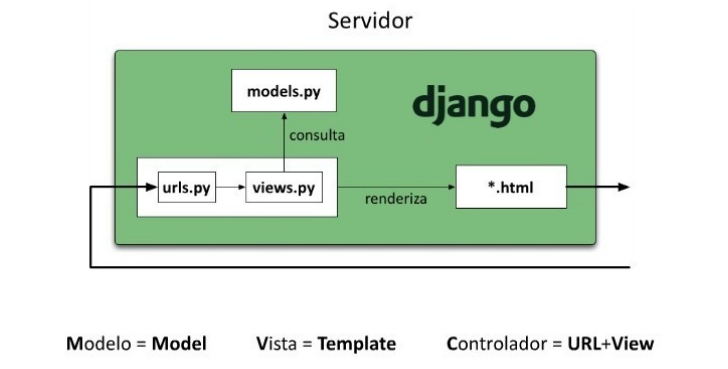
\includegraphics[width=10cm, keepaspectratio]{img/django_MTV.png}
				 	\caption{Patrón MVT Django.}
				 	\label{fig:MTV_Django}
				 \end{figure}
			 
				El proyecto comenzó a desarrollarse en Django 1.9 y ha terminado en la versión Django 1.11.
				
			\subsection{HTML}
				HTML (Hipertextual Markup Lenguaje), es un lenguaje de marcado. Actualmente utilizado para la definición de  estructura básica de los contenidos de una página Web como vídeos, figuras, iframes... \\
				
				Publicado inicialmente en 1991, su historia se remonta a 1980, cuando Tim Berners-Lee propuso un nuevo sistema para compartir documentos. Actualmente se ha impuesto como el estándar, definido por el World Wide Web Consortium (W3C), el cual ha ido evolucionando versión a versión adoptando todas las nuevas exigencias que ofrecen las Webs actuales en el campo de los recursos multimedia y de interactividad. Actualmente la última versión oficial es HTML 5, la cual proporciona soporte nativo de audio y vídeo, inclusión de la etiqueta canvas, entre otras mejoras.\\
				
				HTML se desarrolla por etiquetas o tags, dentro de las cuales se pueden incluir cada uno de los elementos que conforman una página Web. Dispone de cierta capacidad de aportar estilo y lógica pero estas generalmente se delegan en CSS y JavaScript.
			\subsection{CSS}
				CSS (Cascade Style Sheet), es un lenguaje de reglas en cascada utilizado para dotar de diseño a elementos. El cual define, como se mencionó anteriormente, la estética de un documento HTML y por lo tanto de una página Web. Permite crear webs atractivas y responsivas, esto es, que se adapten al dispositivo en que están siendo vistas, ya sean, por ejemplo, tabletas, ordenadores o móviles.\\
				
				Permite mover todas las reglas de estilo
				( tamaños de fuente o imágenes, colores, responsividad de elementos a ciertas resoluciones...) a documentos *.css, evitando así redundancia en documentos *.html, mejorando así la modularidad e independencia dentro de un proyecto.
			\subsection{JavaScript}
				JavaScript es un lenguaje de programación ligero, interpretado, orientado a objetos y dinámico. Utilizado principalmente como lenguaje de scripting para paginas Web, en este campo su papel principal se centra en el desarrollo de lógica en la parte del cliente: acceso al Document Object Model(DOM) de la web, modificación de etiquetas HTML, generación de gráficos en Canvas o gestión de cookies.
				Permite crear nuevo contenido dinámico, así como controlar archivos multimedia y gracias al uso de API's (Aplication Programming Interface), proporciona a JavaScript de más funcionalidades.
				
				\begin{figure}[H]
					\centering
					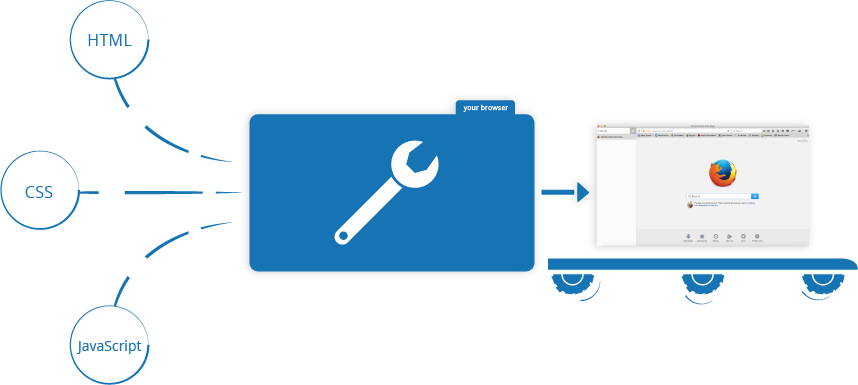
\includegraphics[width=10cm, keepaspectratio]{img/html_css_js.png}
					\caption{Tecnologías web.}
					\label{fig:HTML_CSS_JS}
				\end{figure}
				
				
		\section{Bases de datos}
			\subsection{SQLite}
				SQLite es una librería ligera, rápida y fiable desarrollada en C. Siendo actualmente el motor de bases de datos SQL más usado en el mundo, utilizado en gran parte de los dispositivos móviles y ordenadores, además de venir de serie en muchas aplicaciones, por ejemplo, Django.\\
				
				
				No necesita de de un servidor para funcionar, hecho por el cual su integración y despliegue es sencillo, basado en lectura y escritura en un fichero *.sqlite para almacenar toda la información de una base de datos, este fichero es multiplataforma pudiendo así ser migrado entre distintos sistemas de manera muy sencilla. Con un tamaño máximo de 140 terabytes.
				
			\subsection{MongoDB}
				MongoDB es una base de datos NoSQL distribuida, documental (almacenando la información en ficheros BSON, muy similares a JSON), de código abierto y diseñada para ofrecer un nivel productivo alto.\\
				
				Debido a esta estructura, la velocidad en las consultas es muy alta, convirtiéndose así en una base de datos ideal para trabajar con grandes cantidades de información que vayan a ser consultados muy frecuentemente.\\
				
				La escalabilidad de MongoDB es muy sencilla, puesto que se ejecuta en clusters, podrá escalar horizontalmente contratando más máquinas, aumentando así la capacidad de procesamiento. Es una base de datos muy utilizada en la industria.
			\subsection{ElasticSearch}
				Elasticsearch es una base de datos. Junto a LogStash y kibana, los tres proyectos open source, forman el Stack ELK. Mediante una simple API Rest realiza consulta, borrado y actualización de documentos. Haciendo uso de objetos JSON tanto para las consultas como para las respuestas de estas, lo que la hace muy fácil de usar e integrar en sistemas productivos ya existentes.\\
				
				Basada en Lucene(API para recuperación de información), gracias a esto, permite almacenar información como datos de geolocalización así como realizar búsquedas de texto y auto-completado es muy sencillo.\\
		
				Organizado en nodos, permitirá aumentar la potencia a medida que la demanda de recursos crezca.\\
				
				Datas sus capacidades de almacenar información preparada en índices previamente creados, la consulta de documentos es muy ágil puesto que evitamos búsquedas en indices no deseados, gracias a esto, se ha convertido en uno de los buscadores de texto más importantes, utilizado por gigantes de Internet como Facebook, Netflix o Github.

			\begin{figure}[H]
				\centering
				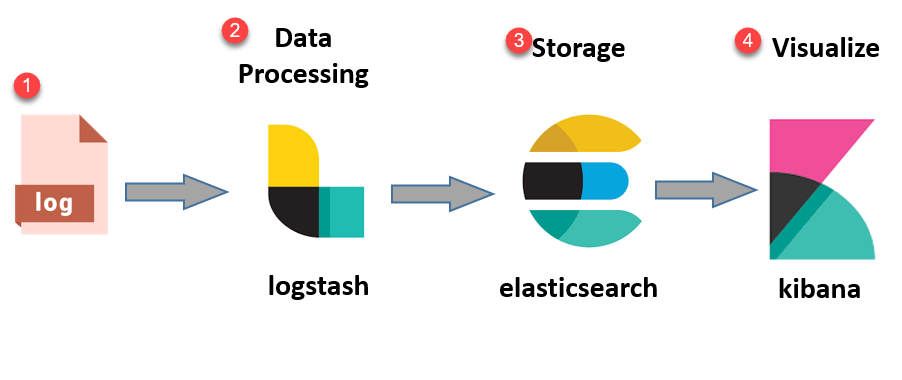
\includegraphics[width=10cm, keepaspectratio]{img/ELK_Stack.png}
				\caption{Stack ELK.}
				\label{fig:MTV_Django}
			\end{figure}
		
		\section{Tecnologías de visualización}
			\subsection{Matplotlib}
				Matplotlib es una librería de Python que se encarga de la generación de visualizaciones tanto estáticas como animadas. \\
				
				Proporciona gran variedad de gráficas como mapas de calor, gráficas de barras, histogramas... recordando a Matlab. Ofrece cierta capacidad de estilo y puede ser utilizada junto a otras librerías, para generar gráficos aún más complejos y enriquecidos como mapas geográficos en los que se representarán datos mediante datos de latitud y longitud. \\
				
				Matplotlib almacena las gráficas en Figuras, cada una contiene los ejes en los que se representarán los datos, estos ejes pueden ser de múltiples tipos, ya sean coordenadas x-y, x-y-x para una representación en tres dimensiones o un eje polar.\\
							
				Estas visualizaciones o gráficos podrán ser mostrados en una nueva ventana si utilizamos la librería en un script o ser renderizadas y devueltas como imagen PNG para su posterior muestra en el servicio Web haciendo uso de la etiqueta HTML <img></img>
			\subsection{Kibana}
				Como se comentó anteriormente, el Stack ELK está compuesto por Kibana como motor de búsqueda, procesador de datos y generador de visualizaciones entre otras muchas funcionalidades.\\
				Gracias a su aplicación frontend, la creación de gráficas se simplifica mucho sin ser necesaria la codificación de estas. \\
				Mediante configuración, filtrado y selección de los datos indexados en ElasticSearch se pueden crear múltiples tipos de visualizaciones interactivas (gráficos de barras, gráficos circulares, tablas, histogramas y mapas), y posteriormente ser agrupadas en tableros o Dashboards, los cuales permiten la visualización y posterior filtrado de grandes cantidades de información de forma simultanea y sencilla.\\
				Permite el procesado de los documentos ya indexados en ElasticSearch para crear nuevos campos dinámicos que podrán ser utilizados y representados posteriormente en visualizaciones y estadísticas.
				
	\chapter{INTEGRACIÓN DE MONGODB Y MATPLOTLIB EN KIBOTICS}
		En este capítulo se describe el estado inicial de Kibotics Webserver, tanto arquitectura de la aplicación web como tecnologías ya utilizadas. Además, se explica la implementación de MongoDB como base de datos, y de Matplotlib como generador de gráficas.
		\section{Estado inicial de Kibotics Webserver}
			En esta sección se describe la arquitectura que poseía Kibotics Webserver al comienzo del desarrollo de este proyecto.
			\subsection{Arquitectura}
				Kibotics Webserver es un servicio web desarrollado en Django. Compuesto por varias partes:
								\begin{itemize}
					\item Kibotics Webserver: Servicio web desarrollado en Django, es el centro de Kibotics y el generador de los logs sobre los que se trabajará en este proyecto fin de carrera.
							
					
					\item Kibotics websim: Simulador robótico que se ejecuta unicamente en el lado del cliente. Desarrollado en herramientas como A-Frame, HTML5, JavaScript, entre otras, permite a los usuarios aprender los fundamentos de la programacón robótica y visión artificial.

					
				\end{itemize}
				
				\begin{figure}[H]
					\centering
					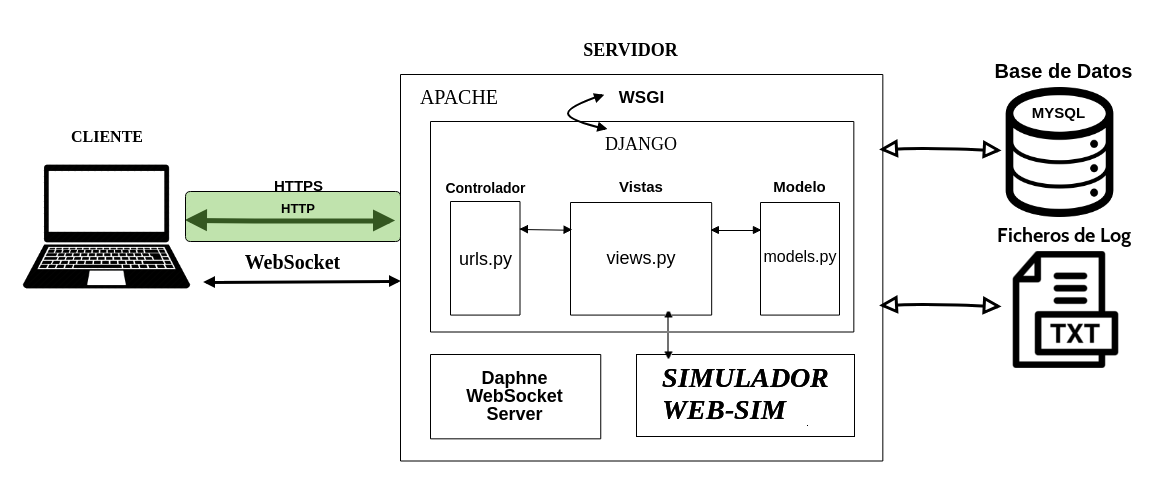
\includegraphics[width=13cm, keepaspectratio]{img/esquema_Kibotics.png}
					\caption{Arquitectura Kibotics.}
					\label{fig:arquitectura_kibotics}
				\end{figure}
			
				Cuando un usuario accede a la plataforma lo hace a través del protocolo HTTPS hacia el servidor Django principal. Este servidor es el orquestador de eventos que tienen lugar en el resto de máquinas.
				\begin{figure}[H]
					\centering
					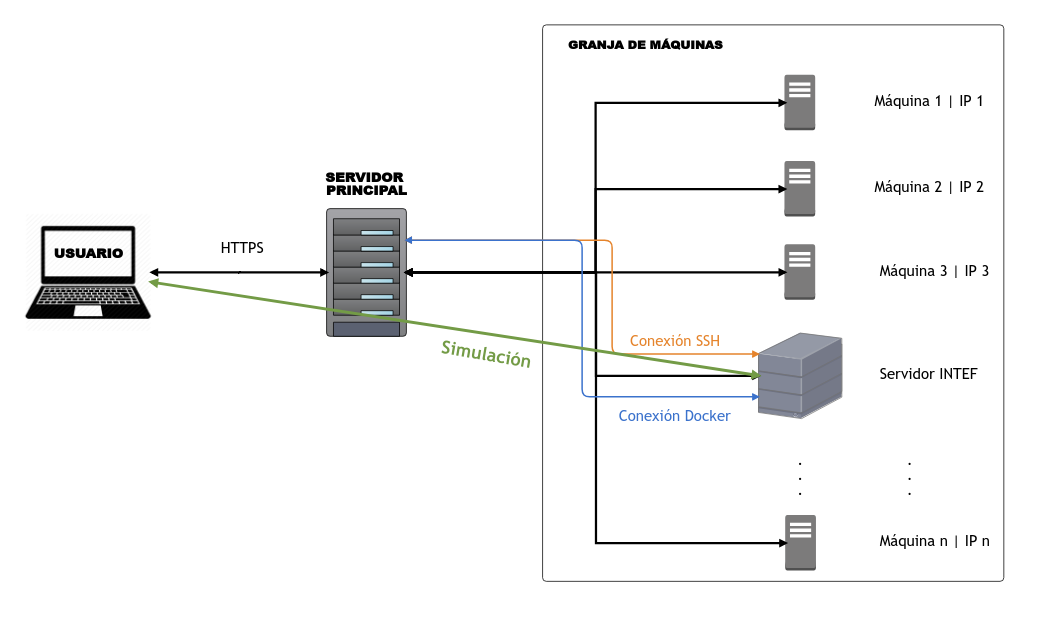
\includegraphics[width=11cm, keepaspectratio]{img/kibotics-infraestructura.png}
					\caption{Infraestructura Kibotics.}
					\label{fig:infraestructura_kibotics}
				\end{figure}
				El centro de Kibotics son las simulaciones. Una simulación está compuesta principalmente de dos partes: el código que programa el estudiante (izquierda) y la ventana de simulación (derecha), en la que el usuario verá su código ejecutado en tiempo real.

				\begin{figure}[H]
					\centering
					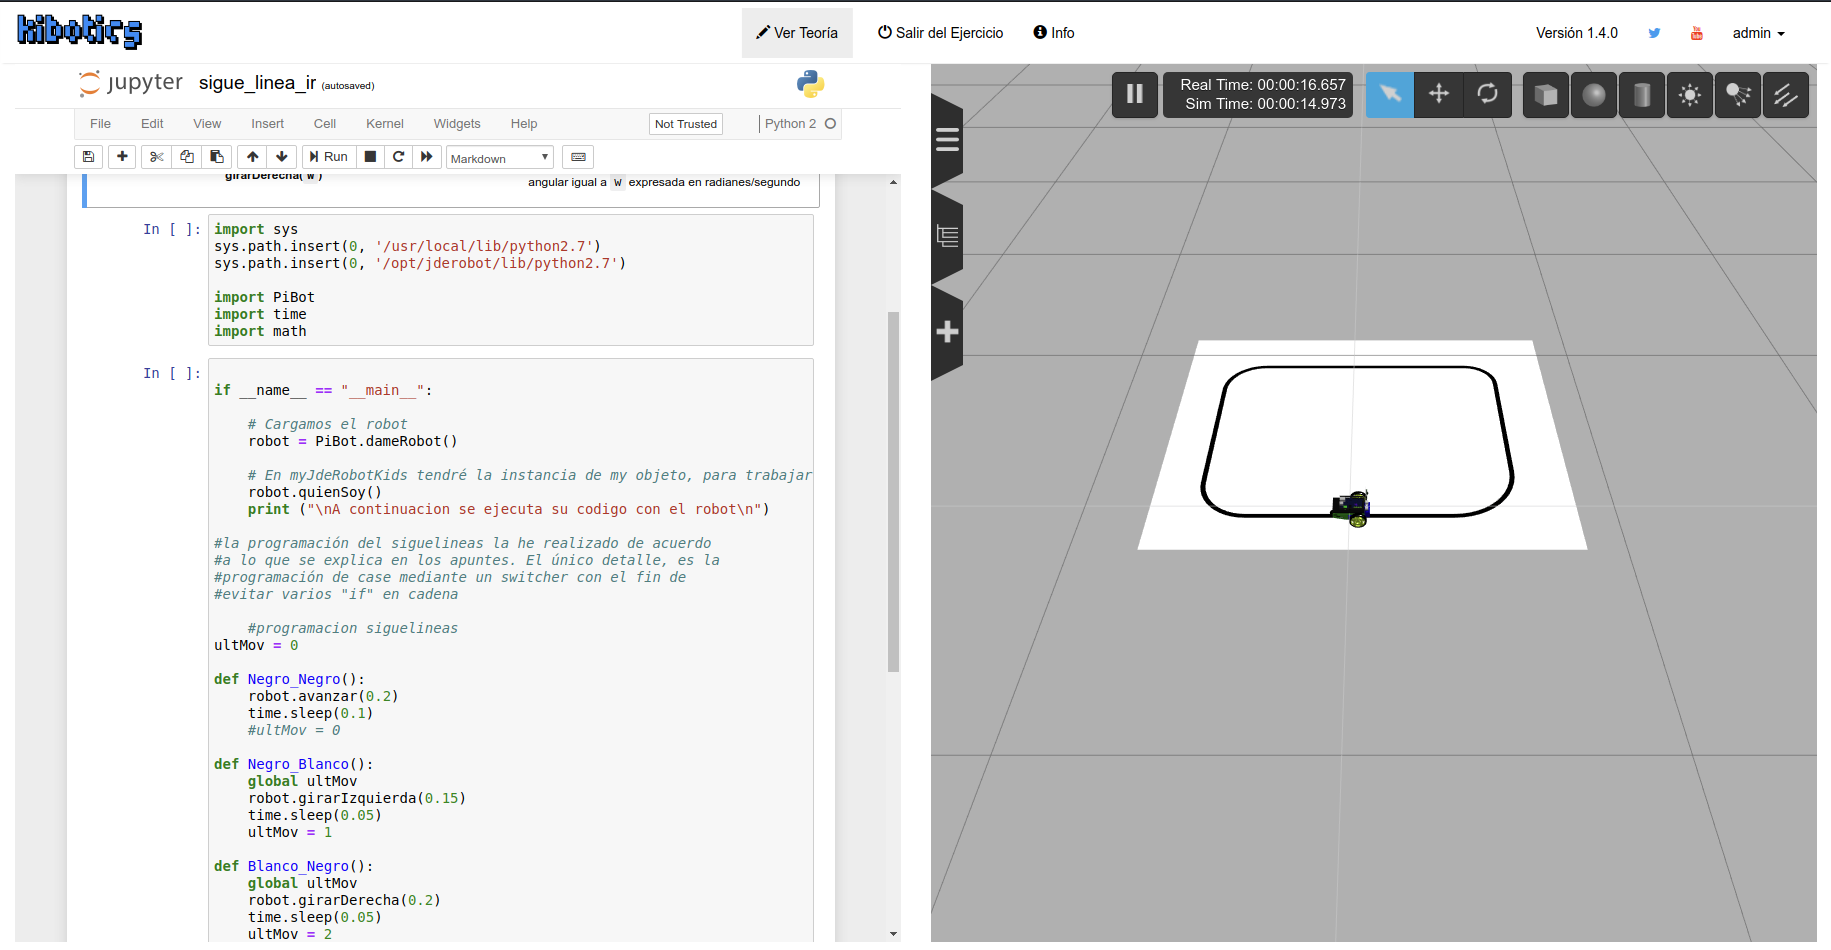
\includegraphics[width=15cm, keepaspectratio]{img/simulacion_kibotics.png}
					\caption{Simulador Kibotics.}
					\label{fig:simulacion_kibotics}
				\end{figure}

			\subsection{Logs}
			Los logs generados por la aplicación Django se guardan en una serie de archivos indexados en el servidor con el formato YYYY-MM-DD-log.txt. Teniendo así, un fichero por día con todos los eventos registrados.
			
			Esta metodología disponía de un sistema numeral de códigos para identificar el evento que había generado cada registro de log. Cada campo de un mismo registro estaba separado por la cadena de caracteres "\ |\ ".\\
			
			Estos códigos y su estructura son los siguientes:
			\begin{itemize}
				\item Log in: "1 | date | user name | user IP | HTTP\_USER\_AGENT"
				\item Log out: "2 | date | user name | user IP | HTTP\_USER\_AGENT"
				\item Comienzo ejecicio: "3 | date | user name | user IP | simulation type | exercise ID | host IP | HTTP\_USER\_AGENT"
				\item Fin ejecicio: "4 | date | user name | user IP | simulation type | exercise ID | host IP | HTTP\_USER\_AGENT"
				\item Error 500: "5 | 500 Internal Server Error"
			\end{itemize}
			Estos log, se generaban en el servicio Django yse guardaban en los ficheros con sentencias Python similares a la siguiente:
			
			\begin{Verbatim}[tabsize=4]
log = open(DIRECTORY + "/logs/" + str(date.today()) + "-log.txt", "a")

traze = "1 | " + str(datetime.now().strftime("%d/%m/%Y %H:%M:%S")) 
+ " | " + username + " | " + client\_ip  + " | " + user\_agent + "\\n"\\

log.write(traze)

log.close()	
			\end{Verbatim}
			
			Además de estos logs, se disponía de los generados de forma automática por Apache. El cual, separa los eventos registrados en dos ficheros, uno con la salida general de la aplicación, asociada a los prints y excepciones producidas. Y el otro, es un archivo de acceso al servidor que muestra las peticiones HTTP que este ha recibido.
		\section{Desarrollo local}
			En está sección se describe la evolución que han sufrido los logs de la aplicación. Así como una primera prueba de concepto de la herramienta de analíticas.
			\subsection{MongoDB en Kibotics Webserver}
			Kibotics webserver disponía de una tecnología muy primitiva de trazabilidad, con limitados eventos y una distribución en ficheros txt. La cual, limitaba la explotación masiva de estos datos para la generación de estadísticas útiles.\\
			
			En Kibotics se espera un crecimiento muy notable en los usuarios. Por lo tanto, la capacidad de procesamiento, almacenamiento y consulta de los logs debía aumentar, haciendo uso de ficheros de texto plano no se podrá conseguir la velocidad de procesamiento necesaria. \\
			Se decide cambiar a un motor de bases de datos, MongoDB, una base de datos externa a Django, a la que se realizarán consultas de Python mediante la librería pymongo. La cual ofrece las herramientas de consulta y guardado necesarias para una interacción ágil con MongoDB.\\
			
			Para realizar esta migración de tecnología, es necesario primero instalar MongoDB:
			
			\begin{Verbatim}[tabsize=4]
$ sudo apt-get install mongodb-org
			\end{Verbatim}

			
			Una vez instalado, es necesario iniciar el proceso para levantar el servicio MongoDB:
			
			\begin{Verbatim}[tabsize=4]
$ sudo systemctl start mongod
			\end{Verbatim}
			
			Adicionalmente a esto, podemos reiniciar o parar el servicio con los siguientes comandos respectivamente:
			
			\begin{Verbatim}[tabsize=4]
$ sudo systemctl restart mongod
$ sudo systemctl stop mongod
			\end{Verbatim}
			
			Con el servicio MongoDB ya instalado lo único necesario para completar la migración es modificar las sondas para evitar que escriban en ficheros. Haciendo uso de la librería pymongo la tarea se simplifica mucho.
			Importamos la librería y abrimos la conexión con la base de datos, para ello: 
			
			\begin{Verbatim}[tabsize=4]
import pymongo
myclient = pymongo.MongoClient("mongodb://localhost:27017/")
mydb = myclient["kiboticsDDBB"]
			\end{Verbatim}
			
			Ya con las conexiones necesarias realizadas, las sondas se transforman a, por ejemplo, las de nueva sesión y simulación:
			\begin{Verbatim}[tabsize=4]
# Nueva sesión
mydict = {
	"date" : datetime_object_test, 
	"username" : "USERNAME_TEST", 
	"client_ip" : "CLIENT_IP_TEST", 
	"user_agent" : "USER_AGENT_TEST"
}
mydb["newSession"].insert_one(mydict)


# Nueva simulación
mydict = {
	"date" : datetime_object, 
	"username" : "USERNAME_TEST", 
	"client_ip" : "CLIENT_IP_TEST", 
	"simulation_type" : "SIMULATION_TYPE_TEST",
	"exercise_id" : "EXERCISE_ID_TEST",
	"host_ip" : "HOST_IP_TEST",
	"container_id" : "CONTAINER_ID_TEST",
	"user_agent" : "USER_AGENT_TEST"
}
mydb["newSimulation"].insert_one(mydict)
			\end{Verbatim}

			Con estos pasos, el logueo en la nueva base de datos MongoDB está completa, para recuperar la información y tratarla en python, una vez más, haciendo uso de pymongo las Queries de búsqueda serán:
		
		
			\begin{Verbatim}[tabsize=4]
# Query nueva sesión
dataNSES = mydb["newSession"].find({
	"username" : {'$regex' : "USERNAME_TEST"}, 
	"date" : {'$lte': first_day_test, '$gte': last_day_test}
});

# Query fin de sesión	
dataESES = mydb["endSession"].find({
	"username" : {'$regex' : "USERNAME_TEST"}, 
	"date" : {'$lte': first_day_test, '$gte': last_day_test}
});

# Query nueva simulación
dataNSIM = mydb["newSimulation"].find({
	"username" : {'$regex' : "USERNAME_TEST"}, 
	"date" : {'$lte': first_day_test, '$gte': last_day_test}
});

# Query fin de simulación
dataESIM = mydb["endSimulation"].find({
	"username" : {'$regex' : "USERNAME_TEST"},
	"date" : {'$lte': first_day_test, '$gte': last_day_test}
});

			\end{Verbatim}	
			
			Como se puede observar estas queries o sentencias de búsqueda filtran tanto por usuarios como por rangos de fechas. Esto aporta mucha flexibilidad para posteriormente simplemente los datos necesarios y evitar tener q recorrer ficheros extra descartando registros de log.
			
			\subsection{Matplotlib en Kibotics Webserver}
			Matplotlib es una librería Python de generación de gráficos. Haciendo uso de ella, se han generado todas las visualizaciones necesarias para el primer prototipo.\\
						
			Estas visualizaciones inicialmente se han separado en dos secciones, analíticas de simulaciones y sesiones, ambas pueden ser filtradas tanto por usuarios como rangos de fechas.\\
			
			Con el guardado de datos que se ha realizado surge un problema inicial, los datos de inicio y fin, tanto para las sesiones como para las simulaciones, están separados en distintas tablas de MongoDB. Por lo tanto, para hacer una relación entre ellos es necesario cruzarlos en Python para unificarlos en un único evento de sesión o simulación. \\
			Para esto, se creó la funcionalidad para unificar estos registros para que proporcionasen información más útil:
			
			\begin{Verbatim}[tabsize=4]
def formatDatesUser(newData, endData):
	USERS = newData.distinct("username")
	newData.sort([('Username', -1), ('date', -1)])
	endData.sort([('Username', -1), ('date', -1)])
	Dict = {}
	
	for user in USERS:
		for d in newData:
			for dd in endData:
				if(dd['username'] == d['username'] == user):
					if(d['date']<dd['date']):
						if(user not in Dict):
							Dict[user] = {d['date'] : 
								{
									"totalTime" : dd['date']-d['date'],
									"endTime" : dd['date']
								}
							}
						else:
							Dict[user].update({d['date'] : 
								{
									"totalTime" : dd['date']-d['date'],
									"endTime": dd['date']
								}
							})
				break;
			endData.rewind()
		newData.rewind()

return Dict
			\end{Verbatim}
			
			Este código extrae todos los usuarios y posteriormente recorre los registros de principio a fin buscando por el campo hora hasta encontrar la inmediatamente siguiente de cierre. Nos devolverá un diccionario de diccionarios con cada uno de los eventos sesión/simulación para cada usuario del que haya ocurrencias.\\
			
			La clave de este diccionario serán los usuarios. El valor, será otro diccionario con las fechas de comienzo y fin del evento así como su duración.\\
			
			Un ejemplo de respuesta sera:
			
			\begin{Verbatim}[tabsize=4]
{
	"USERNAME_TEST_1" : {
		start_date_1 : {
			"endTime" : end_date_1,
			"totalTime" : end_date_1 - start_date_1
		},
		start_date_2 : {
			"endTime" : end_date_2,
			"totalTime" : end_date_2 - start_date_2
		},
		
		...
		start_date_N : {
			"endTime" : end_date_N,
			"totalTime" : end_date_N - start_date_N
		},
	},
	
	...
	"USERNAME_TEST_N" : {
		start_date_1 : {
			"endTime" : end_date_1,
			"totalTime" : end_date_1 - start_date_1
		},
		start_date_2 : {
			"endTime" : end_date_2,
			"totalTime" : end_date_2 - start_date_2
		},
		
		...
		start_date_N : {
			"endTime" : end_date_N,
			"totalTime" : end_date_N - start_date_N
		},
	}
}
			\end{Verbatim}
			
			Una vez con estos datos más completos, ya se puede enviar a métodos de generación de gráficas, estos tienen una estructura muy similar entre ellos:
	
			\begin{itemize}
				\item Primero, recorrerán los datos de entrada formateandolos a la estructura de ejes necesaria para cada una de las gráficas. Generalmente se compondrá de dos listas o arrays, uno con los datos del eje-X y otro con los referentes al eje-Y. En ciertos casos como el mapa de calor, necesitaremos una matriz de datos para la correcta representación de la información.
				
				\item Segundo, se creará la gráfica y se le añadirán los datos que se formatearon en el punto primero. Este es el paso en el que se explicitará qué tipo de gráfica se insertará para cada caso. Junto a la primera parte, es lo que más cambiará entre métodos.
				
				\item Tercero, se ajustará el diseño de la gráfica para que encaje estéticamente tanto con las otras gráficas generadas para la funcionalidad de analíticas, como con el diseño ya existente en la aplicación.
				
				\item Finalmente, ya generada la gráfica, se guardará la figura en un objeto BytesIO. Este objeto de bytes, se codificará a formato png y se devolverá por la salida del método.
			\end{itemize}
			
			Con estos objetos de imagen ya guardados, lo único que queda es devolverlos por el contexto de la respuesta HTML de Django, que es simplemente un diccionario de variables. Es a este contexto al que la platilla HTML enriquecida de Django accederá para mostrar las imágenes.\\
						
			Un ejemplo de una sección en estas plantillas será:
			\begin{Verbatim}[tabsize=4]
...	
<div class="main">
	<br><br><h2>INICIOS POR DIA DE LA SEMANA</h2>
	<hr/>
	
	<div class='left' >
		<h4>Sesiones</h4><br>
		<img class='analyticsIMG'src="data:image/png;base64, {{ imageWeekSesion }}" 
		alt="Data not loaded properly" width=500 height=auto />
	</div>
	
	<div class='right'>
		<h4>Simulaciones</h4><br>
		<img class='analyticsIMG'src="data:image/png;base64, {{ imageWeekSimulation }}" 
		alt="Data not loaded properly" width=500 height=auto />
	</div>
</div>
...
			\end{Verbatim}
		
		A continuación se puede ver el resultado final, con unos datos de prueba, no productivos. El prototipo nos muestra mucha información acerca de la actividad en la aplicación web.\\
		\begin{figure}[H]
			\centering
			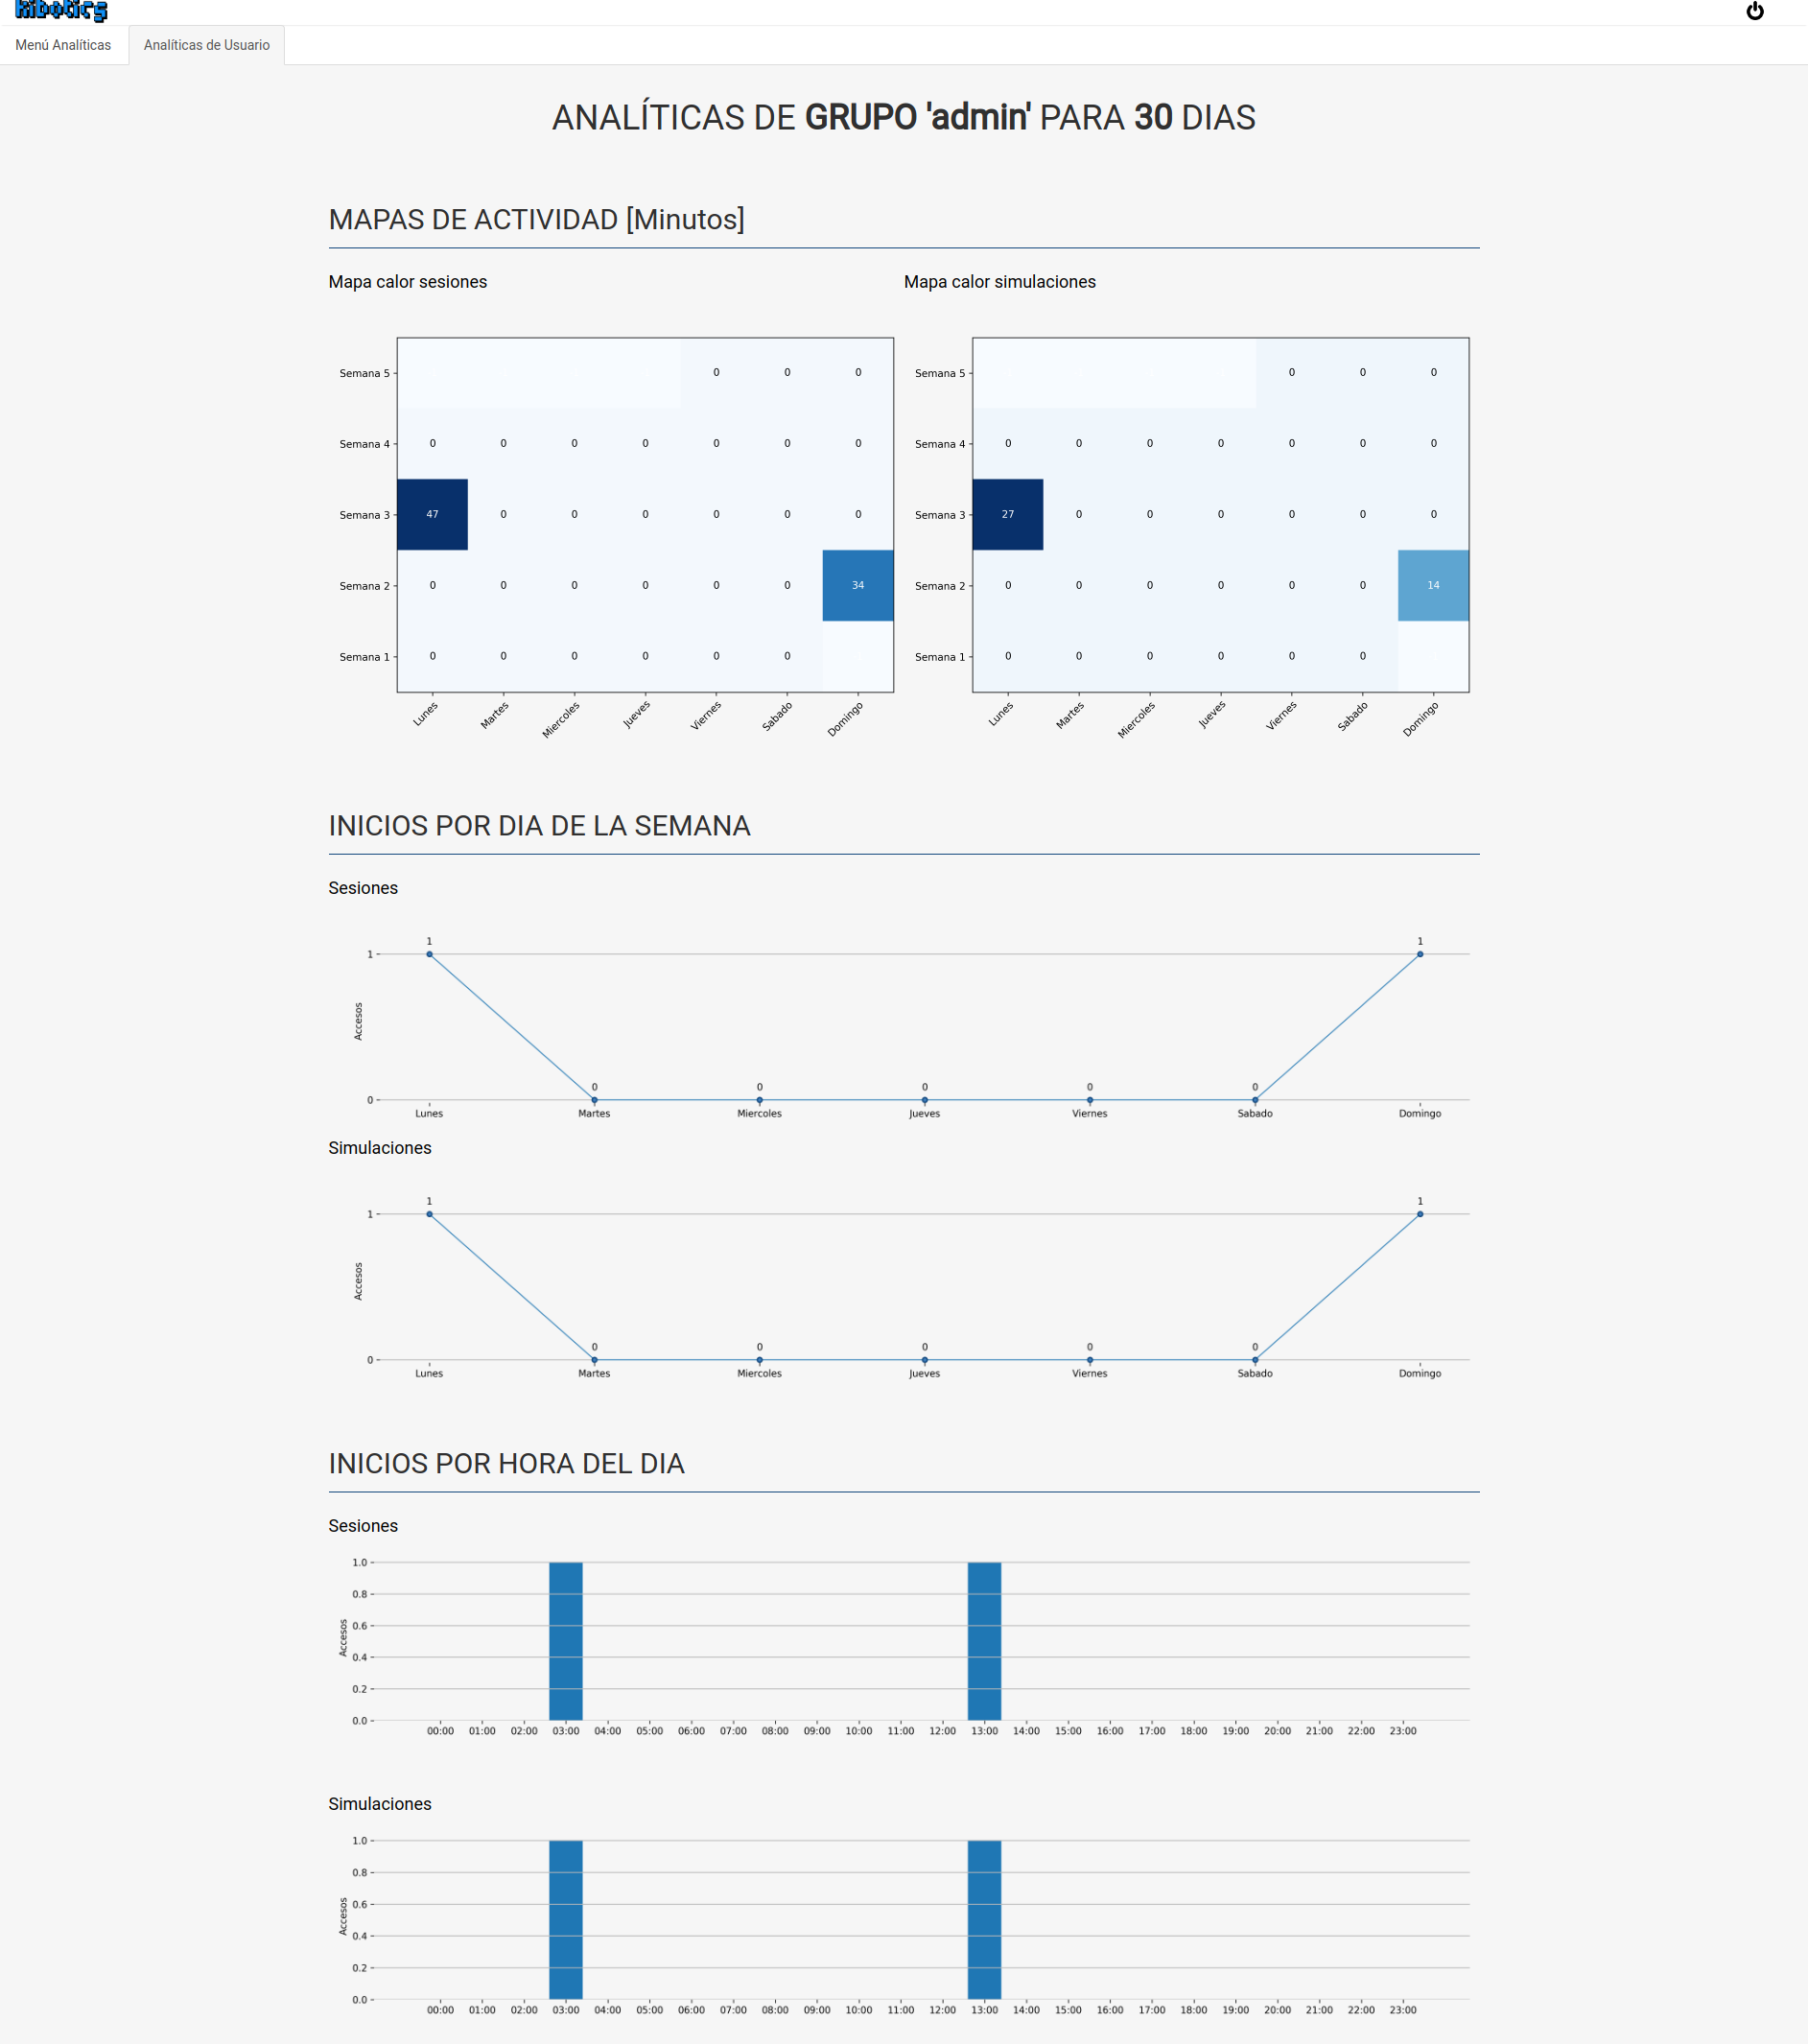
\includegraphics[width=14cm, keepaspectratio]{img/primer_prototipo_1.png}
			\caption{Primer prototipo parte 1.}
			\label{fig:primer_prototipo_1}
		\end{figure}
		En la primera figura, se puede observar una primera parte con un mapa de calor tanto para simulaciones como para sesiones, la cual representa la actividad en minutos para el grupo de usuarios analizado.\\
		En una segunda parte, se representar 4 gráficas más con los accesos a sesiones y simulaciones separadas en dos grupos. Una primera agrupación con los accesos por día de la semana, a continuación, el segundo grupo con accesos divididos por la hora del día a la que fueron realizadas.\\
		
		Por último en la siguiente figura, se representan las dos últimas gráficas. Una primera con los tiempos totales y medios que el grupo de usuarios o usuario ha pasado en cada uno de los ejercicios a los que ha accedido.\\
		
		Finalmente, la última gráfica representa con un mapa geográfico la localización desde la que cada acción se ha realizado.\\
		
		Este primer prototipo es bastante completo pero tiene ciertos inconvenientes. Primero, falta cierta información útil que podría ser representada, como desde que dispositivos acceden los usuarios.\\
		
		Esta gráficas, al estar insertadas como imágenes, carecen de interactividad, la cual sería muy útil para tener información extra o poder realizar mas filtrado de los datos.
		\begin{figure}[H]
			\centering
			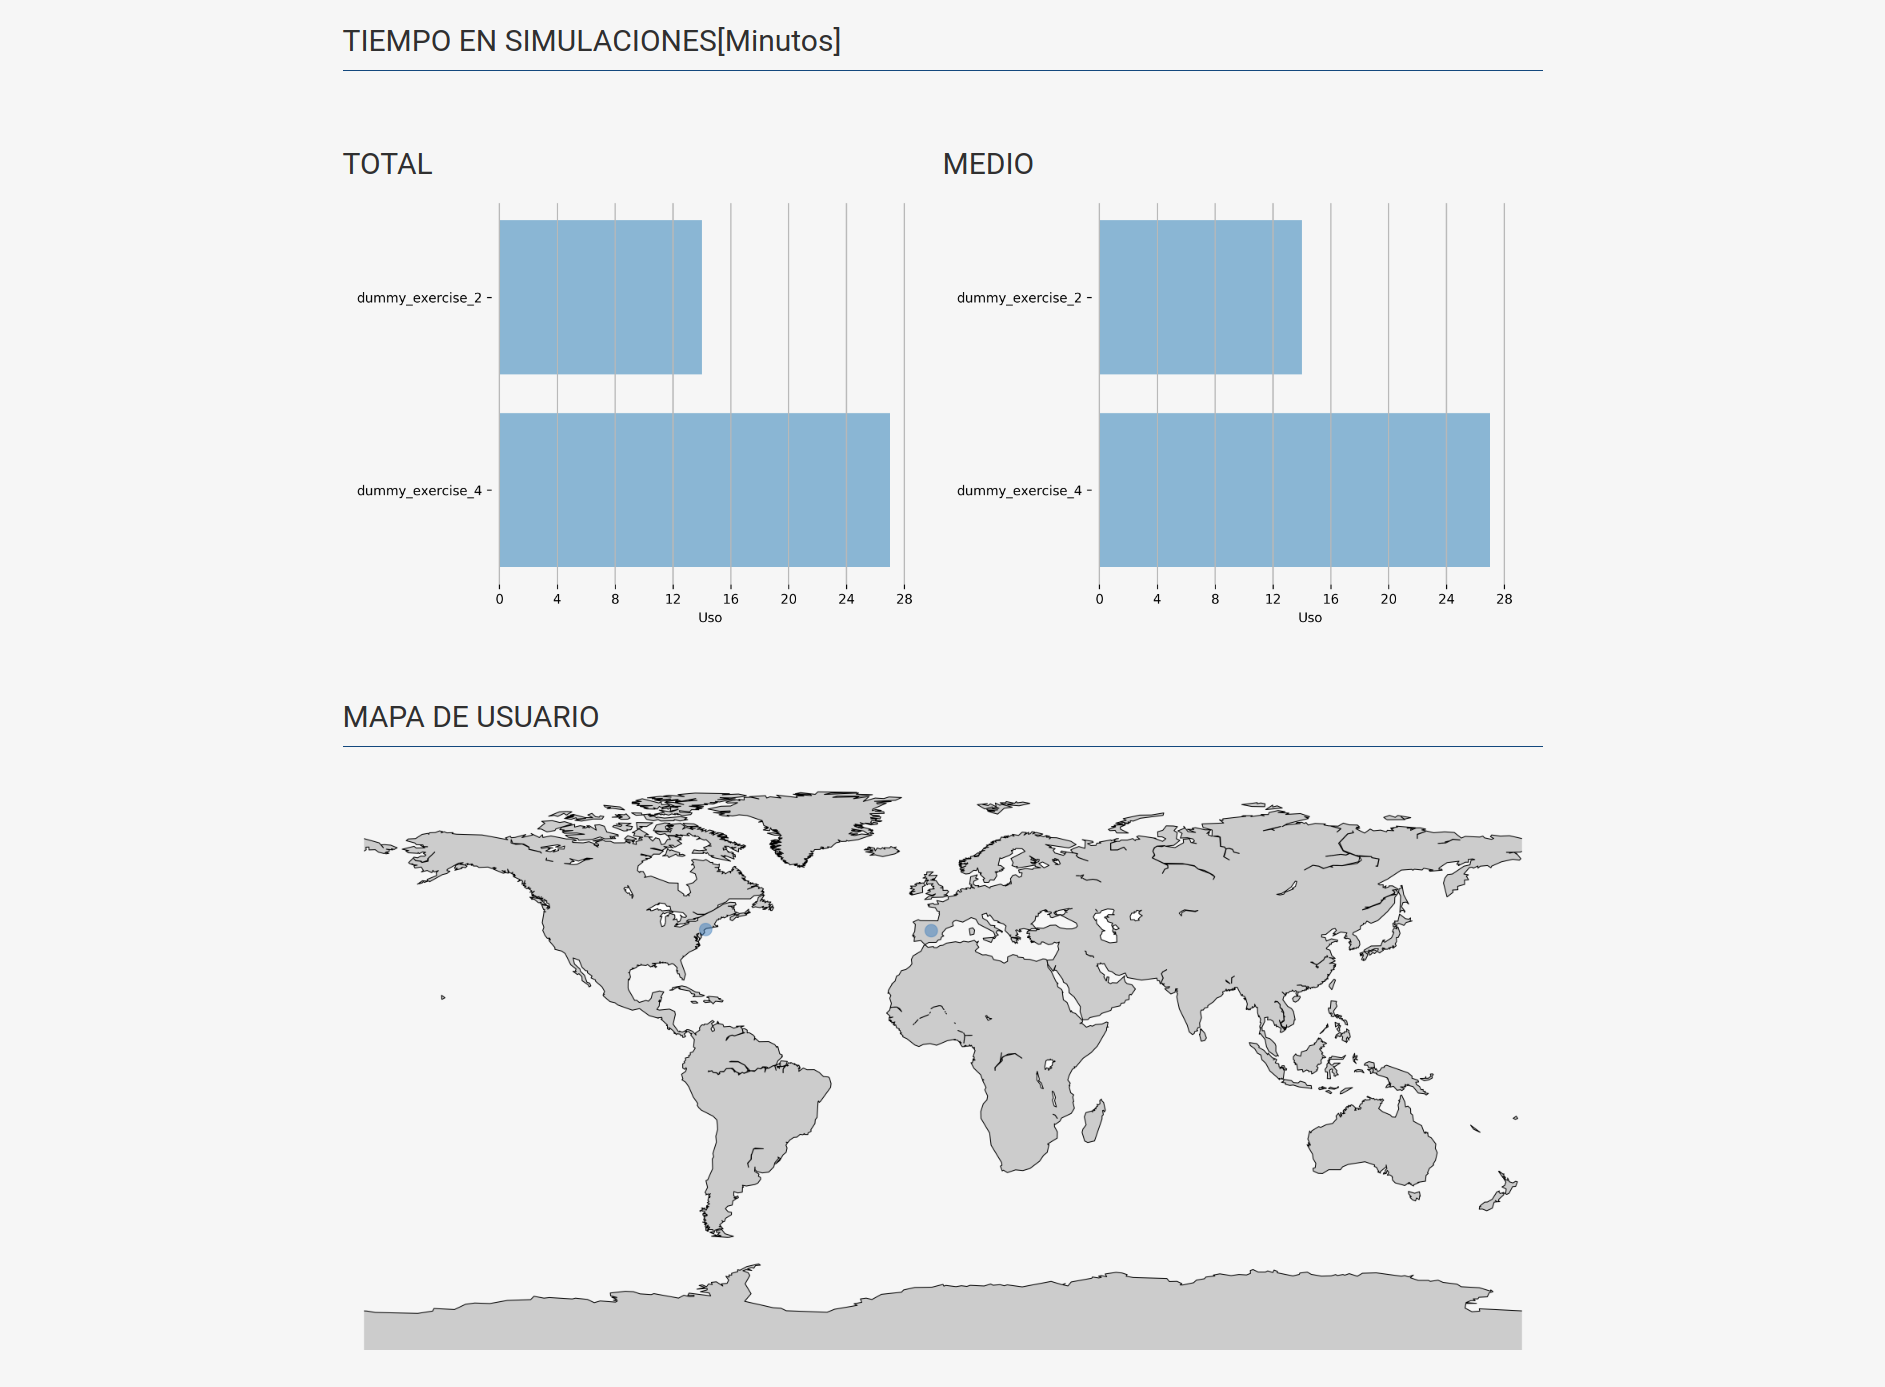
\includegraphics[width=14cm, keepaspectratio]{img/primer_prototipo_2.png}
			\caption{Primer prototipo parte 2.}
			\label{fig:primer_prototipo_2}
		\end{figure}
	
	
	\chapter{INTEGRACIÓN DEL STACK ELK EN KIBOTICS}
		En este capítulo se describen las tecnologías del Stack ELK utilizadas en la versión final desarrollada del módulo de analíticas. Tanto Elasticsearch como base de datos, como Kibana de procesador de datos y generador de gráficas. Además de unos recursos de prueba generados para que futuros desarrolladores dispongan de una instalación sencilla de bases de datos y servicios necesarios.
		\section{Desarrollo local}
			En está sección se describe la evolución que han sufrido los logs de la aplicación. Así como la versión final de la herramienta de analíticas que hará uso del Stack ELK.
			\subsection{ElasticSearch en Kibotics Webserver}
				El primer paso el proceso de migración es el cambio de bases de datos. Para hacer uso del Stack ELK, es necesario sustituir MongoDB por ElasticSearch. Para esto lo primero será instalar e inciar un servicio de Elasticsearch en local.\\
				
				Una vez iniciado el servicio Elasticsearch podremos acceder a los datos indexados en las tablas mediante la interfaz a la que se podrá acceder por la terminal de comandos o de manera más amigable, desde la URL y puerto local que hayamos configurado en la instalación de ElasticSearch.\\
				
				Un ejemplo de llamada para un índice llamado index\_name\_test será la siguiente:
				
				\begin{Verbatim}[tabsize=4]
http://127.0.0.1:9200/index_name_test/_search/?size=1000&pretty
				\end{Verbatim}
				
				El siguiente paso en la migración es la integración de Elasticsearch en Django, se realizará haciendo uso de la librería django\_elasticsearch\_dsl, la cual simplificará esta tarea. La cual, se divide en dos partes principales. Creación de los índices y migración de las sondas de MongoDB a Elasticsearch.\\
				
				
				Este primer paso de creación de índices es similar a la metodología de modelos que posee Django con las estructuras de las bases de datos. Se creará los siguientes índices: 				

				\begin{itemize}
					\item kibotics\_session\_log: En el cual se almacenarán todos los eventos referentes a las sesiones.
					
					\item kibotics\_simulation\_log: En el cual se almacenarán todos los eventos referentes a las simulaciones.
					
					\item kibotics\_error\_log: En el cual se almacenarán todos los eventos referentes a los errores.
					
					\item kibotics\_visit\_log: En el cual se almacenarán todos los eventos referentes a las visitas.
				\end{itemize}				
								
				Aprendiendo de lo aplicado en el primer prototipo y para evitar tener que cruzar datos para el calculo de duraciones de los eventos logueados, tanto en el índice de sesiones como de simulaciones se ha eliminado el campo que registraba la fecha. Para sustituirlo, se han añadido dos nuevos campos los cuales registrarán el inicio y fin de cada evento, unificando así los dos registros de log que se tenían previamente en uno.\\
				
				Por otro lado el campo USER\_AGENT ha sido dividido y sustituido con la información del navegador, dispositivo y sistema operativo con el que cada usuario accederá a la web.\\
				
				Para trabajar en Kibana con mapas es necesario guardar tanto la longitud como la latitud, para lo cual se creará un campo ya existente llamado Geo Point que almacenará en un diccionario ambos campos.\\
								
				Para complementar las nuevas sondas, de las que se a continuación, es necesario la creación de un nuevo índice de visitas, en el que se registrarán los accesos a la pagina principal de la aplicación, estén o no registrados.\\
				
				Un ejemplo de la estructura de uno de estos índices en el fichero Python documents.py es:
				
				\begin{Verbatim}[tabsize=4]
from django_elasticsearch_dsl import Document, Text, Date, Double, GeoPoint, Ip
				
class SessionDocument(Document):
	username = Text()
	start_date = Date()
	end_date = Date()
	duration = Double()
	client_ip = Ip()
	browser = Text()
	os = Text()
	device = Text()
	location = GeoPoint()
	
	class Index:
		name = 'kibotics_session_log'
		settings = {
			'number_of_shards': 1,
			'number_of_replicas': 0
		}		
				\end{Verbatim}
				
					
				Por último, ya solo será necesaria la migración de las sondas de obtención de logs. Para enriquecer las sondas ya existentes, se han añadido nuevas para registrar eventos de visitantes, así como sondas para fin de sesiones/simulaciones (cierre busco de la aplicación, temporizador por inactividad) con el fin de evitar entradas de log sin fecha de fin.\\
				
				Las sondas de inicio de los eventos son similares a las que se tenían anteriormente en MongoDB, por ejemlo:
				
				\begin{Verbatim}[tabsize=4]
SimulationDocument(
	username = "USERNAME_TEST",
	start_date = start_date_object_test,
	end_date = start_date_object_test,
	duration = 0.0,
	client_ip = "CLIENT_IP_TEST",
	simulation_type = "SIMULATION_TYPE_TEST",
	exercise_id = "EXERCISE_ID_TEST",
	browser = "BROWSER_TEST",
	os = "OS_TEST",
	device = "DEVICE_TEST",
	location = {'lat': latitude_double_test, 'lon': longitude_double_test}
).save()
				\end{Verbatim}

				Sin embargo, las sondas de fin de sesión/simulación cambian. Tendrán que buscar en ElasticSearch el último registro de log en el índice para el usuario del cual se quiera actualizar el registro de log y sustituir tanto los campos end\_date como duration. \\
				Esto se realiza gracias al identificador que cada registro indexado posee al cual se le realiza una operación update con los nuevos campos:
				
				\begin{Verbatim}[tabsize=4]
latest_session = Search(index="kibotics_session_log*") \
	.query("match", username=username) \
	.query('match', duration=0) \
	.sort({"start_date": {'order': 'desc'}})[0]

# Update session with leave date and duration
for hit in latest_session:
	duration = datetime.now() - datetime.strptime( \
									hit.start_date, \
	 								"%Y-%m-%dT%H:%M:%S.%f")
	 
	Elasticsearch(settings.ELASTICSEARCH_DSL['default']['hosts']) \
	.update(index = 'kibotics_session_log', 
			id = hit.meta.id,
			body = {"doc": {
						'end_date' : datetime.now(), 
						'duration' : duration.total_seconds()
					}
				}
			)
				\end{Verbatim}
				
				Para comprobar que todos estos campos están siendo creados y actualizados correctamente se puede realizar haciendo consultas tanto por terminal, así como a la API Rest de ElasticSearch que se levantó previamente, accediendo mediante la URL y puerto configurados durante el proceso de instalción.	\\
				
				En esta API, podremos realizar filtrados por campos e índices haciendo uso de expresiones regulares Regex, un ejemplo genérico para uno de los índices de kibotics será:
				
				\begin{Verbatim}[tabsize=4]	
http://127.0.0.1:9200/kibotics_session_log/_search/?size=1000&pretty
				\end{Verbatim}

				En la siguiente figura se puede observar la respuesta que se obtiene a la llamada anterior.
					
				\begin{figure}[H]
					\centering
					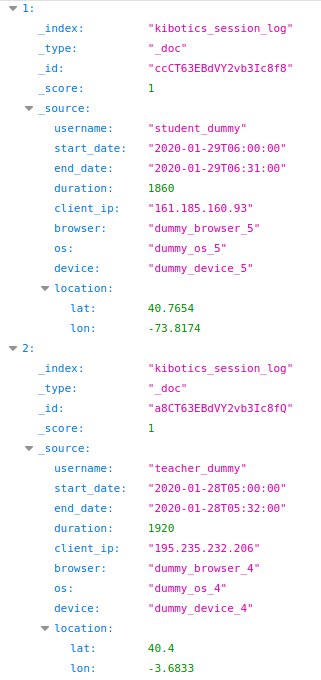
\includegraphics[width=9cm, keepaspectratio]{img/api_elasticsearch.png}
					\caption{API Rest ElasticSeach.}
					\label{fig:api_elasticsearch}
				\end{figure}

			\subsection{Kibana en Kibotics Webserver}
				
				Para acceder a kibana, deberemos primero instalar y ejecutar el servicio. Una vez Kibana está ejecutando podremos acceder a su interfaz gráfica mediante la URL y puerto configurado en la instalación:
				
				\begin{Verbatim}[tabsize=4]	
http://127.0.0.1:5601/app/kibana#/home
				\end{Verbatim}
				
				Ya con datos en ElasticSearch, Kibana nos pedirá que registremos los índices sobre los que queremos obtener soporte y seleccionemos el campo sobre el que se filtrarán temporalmente estos logs. En este caso, el campo start\_date.

				\begin{figure}[H]
					\centering
					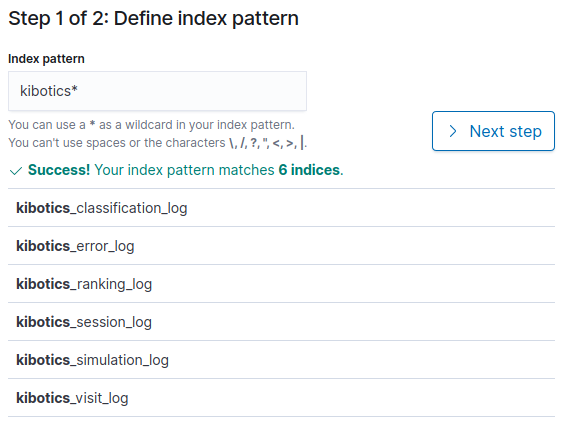
\includegraphics[width=11cm, keepaspectratio]{img/index_pattern_kibana.png}
					\caption{Creación de índices en Kibana.}
					\label{fig:index_pattern_kibana}
				\end{figure}
			
				Configurados todos los índices en Kibana, se podrá tener una primerá visualización de los datos indexados en ElasticSearch en la pestaña Discover de Kibana. En esta pestaña podremos ver todos los logs que estén guardados así como un histograma en el que se podrá ver gráficamente la evolución de los índices. Además, esta sección Discover proporciona la posibilidad de filtrar por rangos de fechas y campos así como se tenía en el primer prototipo de este proyecto.\\
				
				Esta sección ya nos da una primera pincelada de la potencia de procesamiento de Kibana, así como la sencillez de implementación y despliegue.
				\begin{figure}[H]
					\centering
					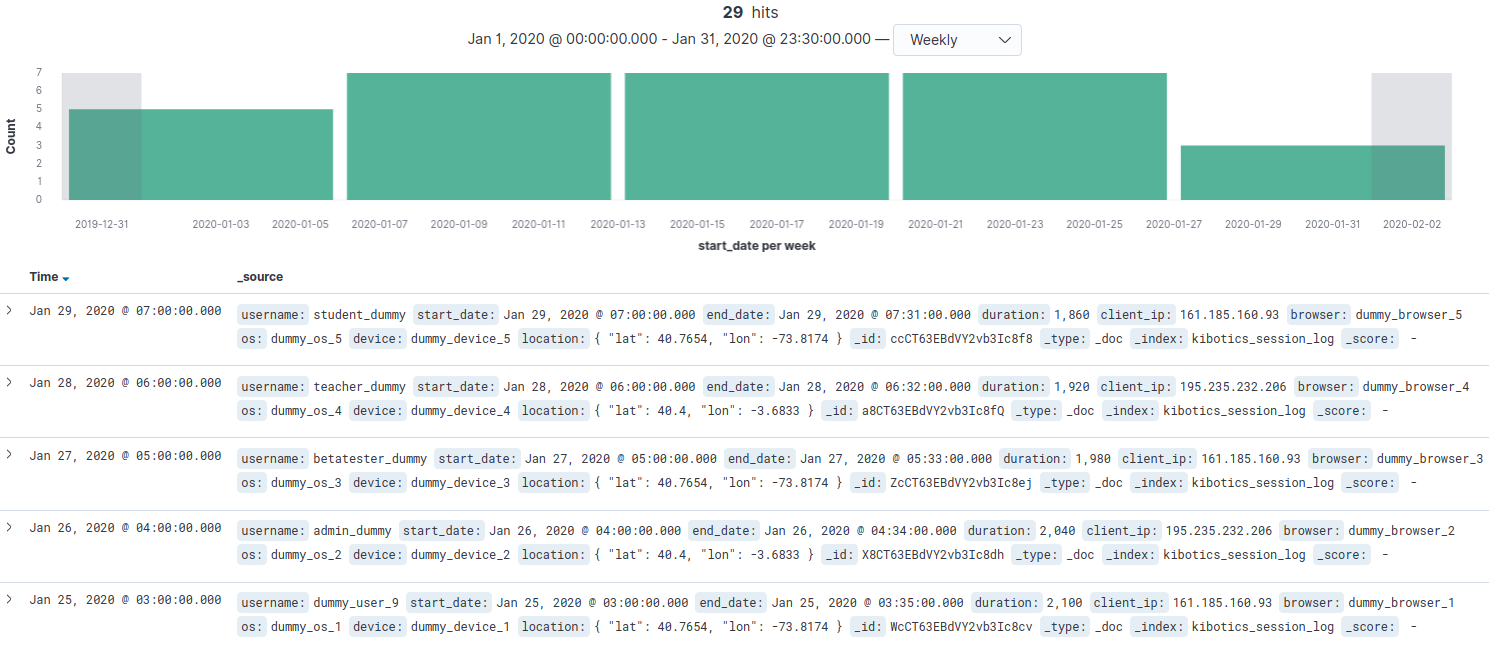
\includegraphics[width=15cm, keepaspectratio]{img/discover_kibana.png}
					\caption{Sección Discover en Kibana.}
					\label{fig:discover_kibana}
				\end{figure}
			
				Kibana ofrece la posibilidad de creación de scripted fields, estos son, campos cuyo valol derivará de otros campos o datos ya indexados, generados en un legunaje muy similar a C llamado painless. Para la versión final de la herramienta necesitaremos crear varios de estos campos para distintas gráficas que se explicarán más adelante como por ejemplo el mapa de calor de actividad.\\
				
				Estos son el día de la semana y la hora del día en que los logs se registraron.
				\begin{Verbatim}[tabsize=4]	
# day_of_week
["", "1 Lunes", "2 Martes", "3 Miercoles", "4 Jueves", "5 Viernes",
 "6 Sabado", "7 Domingo"] [doc['start_date'].value.dayOfWeek]

# hour_of_day
doc['start_date'].value.hourOfDay
				\end{Verbatim}
				
				Con estos campos creados además de los contenidos en los registros de log, Kibana ya dispone de todos los datos necesarios para la creación de las visualizaciones. Para ellos en la sección Visualize, kibana tiene una colección de distintas plantillas gráficas. Las cuales, deberán ser configuradas para representar los datos e índices que sean necesarios.
				
				
				\begin{figure}[H]
					\centering
					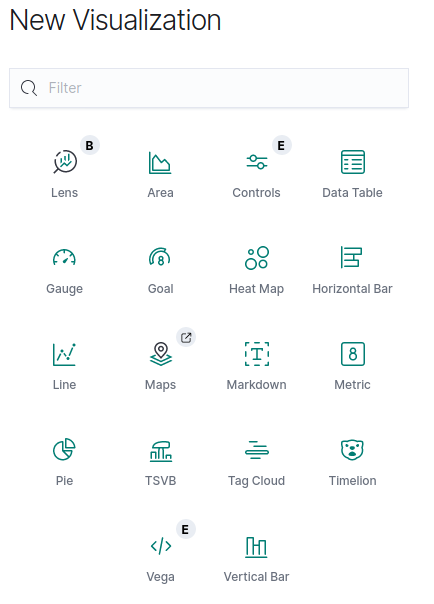
\includegraphics[width=7cm, keepaspectratio]{img/visualization_selector.png}
					\caption{Menú creación de visualizaciones.}
					\label{fig:visualization_selector}
				\end{figure}
			
				Se han creado una amplia selección de visualizaciones. Divididas en dos Dashboards, el primero reservado a los visitantes y el segundo para analíticas de sesiones y simulaciones de usuarios registrados. A continuación se mostrarán las gráficas creadas, así como una breve explicación de lo que representan.
				
				\begin{figure}[H]
					\centering
					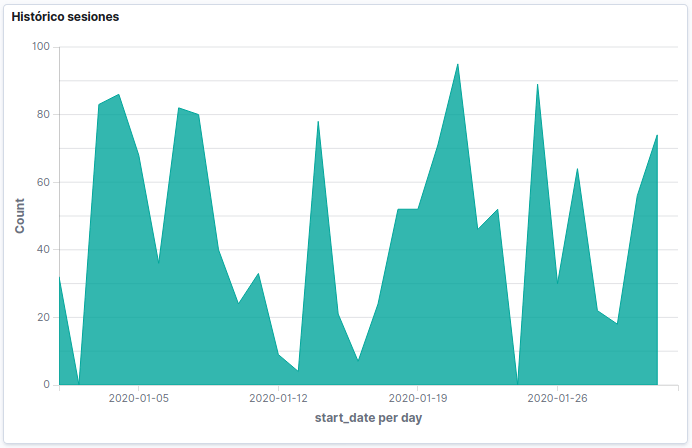
\includegraphics[width=10cm, keepaspectratio]{img/kibana_01_histogram}
					\caption{Histograma}
					\label{fig:kibana_histogram}
				\end{figure}
				Histograma que representará el número de logs registrados en el índice de sesiones para el rango de fechas señalado.
				
				
				\begin{figure}[H]
					\centering
					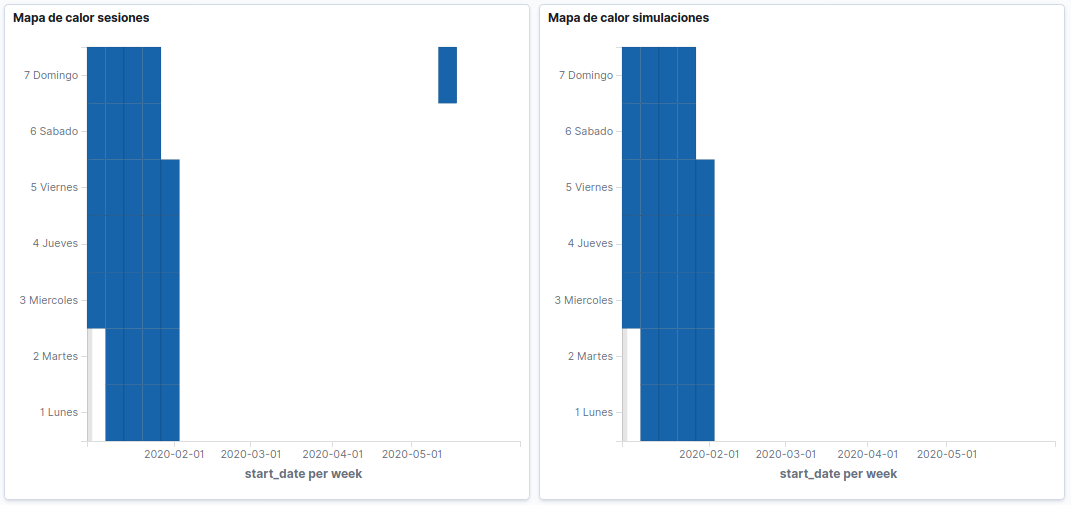
\includegraphics[width=11cm, keepaspectratio]{img/kibana_02_heatMap}
					\caption{Mapa de calor sesiones y simulaciones}
					\label{fig:kibana_heatmap}
				\end{figure}
				Mapas de calor para los índices se sesiones y simulaciones, divididos en columnas por semanas, cada una de ellas en los respectivos días de la semana. Un color más oscuro representará mayor actividad para ese día.\\
				
				\begin{figure}[H]
					\centering
					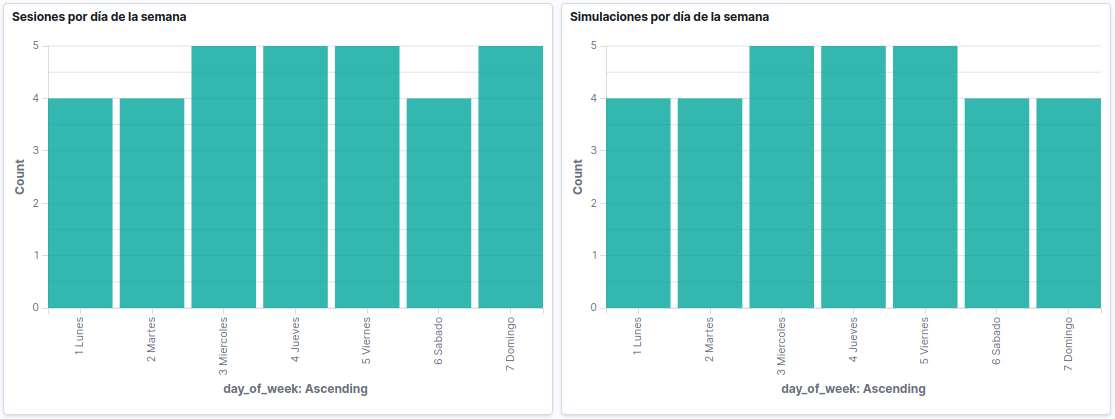
\includegraphics[width=10cm, keepaspectratio]{img/kibana_03_day_of_week}
					\caption{Gráfico de barras por día de la semana}
					\label{fig:kibana_dayofweek}
				\end{figure}
				Gráfica de barras que dividirá los datos filtrados por el día de la semana en que se registraron. Tanto para sesiones como para simulaciones.\\
				
				\begin{figure}[H]
					\centering
					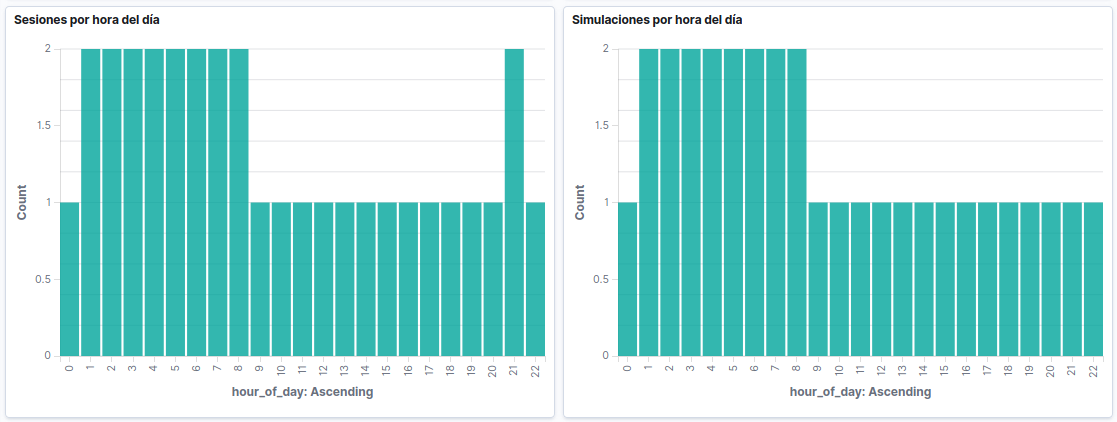
\includegraphics[width=10cm, keepaspectratio]{img/kibana_04_hour_of_day}
					\caption{Gráfico de barras por hora del día}
					\label{fig:kibana_hourofday}
				\end{figure}
				Gráfica de barras que dividirá los datos filtrados por la hora del día en que se registraron. Tanto para sesiones como para simulaciones.\\
				
				\begin{figure}[H]
					\centering
					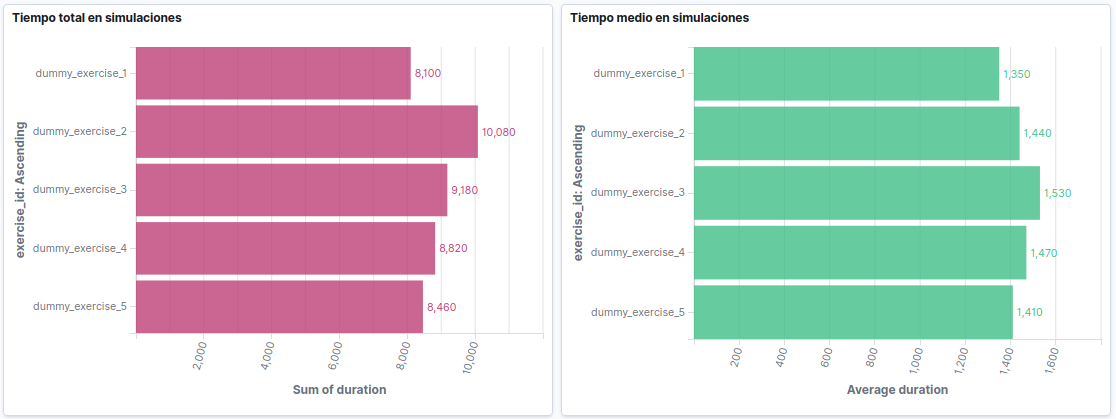
\includegraphics[width=10cm, keepaspectratio]{img/kibana_05_simulations}
					\caption{Gráfico de barras para tiempo total y medio en simulaciones}
					\label{fig:kibana_simulations}
				\end{figure}
				Gráfica de barras que representará el tiempo invertido por los usuarios filtrados en las respectivas simulaciones. El gráfico de la izquierda muestra el tiempo total y el de la derecha el tiempo medio invertido.\\
				
				\begin{figure}[H]
					\centering
					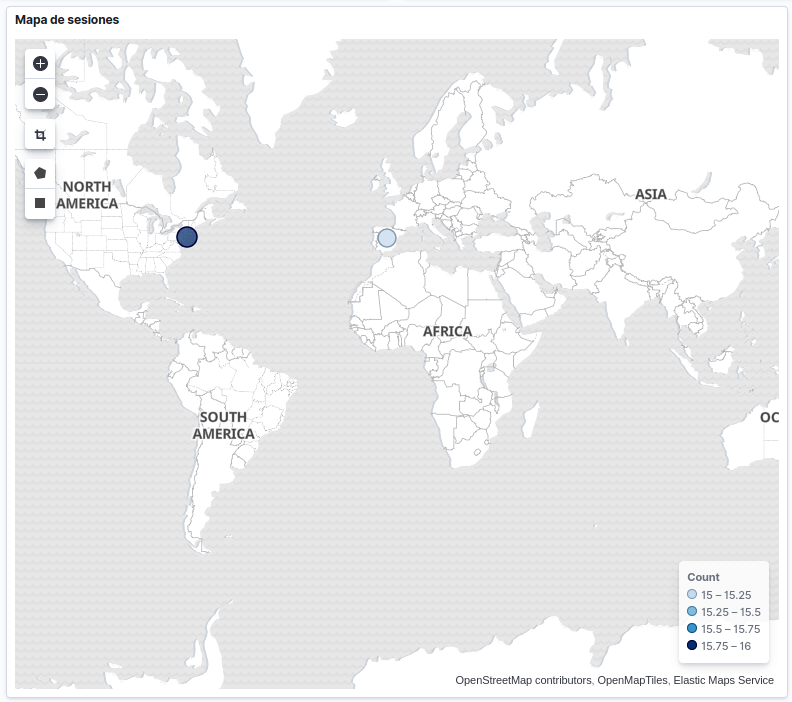
\includegraphics[width=10cm, keepaspectratio]{img/kibana_06_map}
					\caption{Mapa geográfico de sesiones}
					\label{fig:kibana_map}
				\end{figure}
				Representación geográfica de los eventos de sesión ocurridos para el rango de fechas filtrado.\\
				
				\begin{figure}[H]
					\centering
					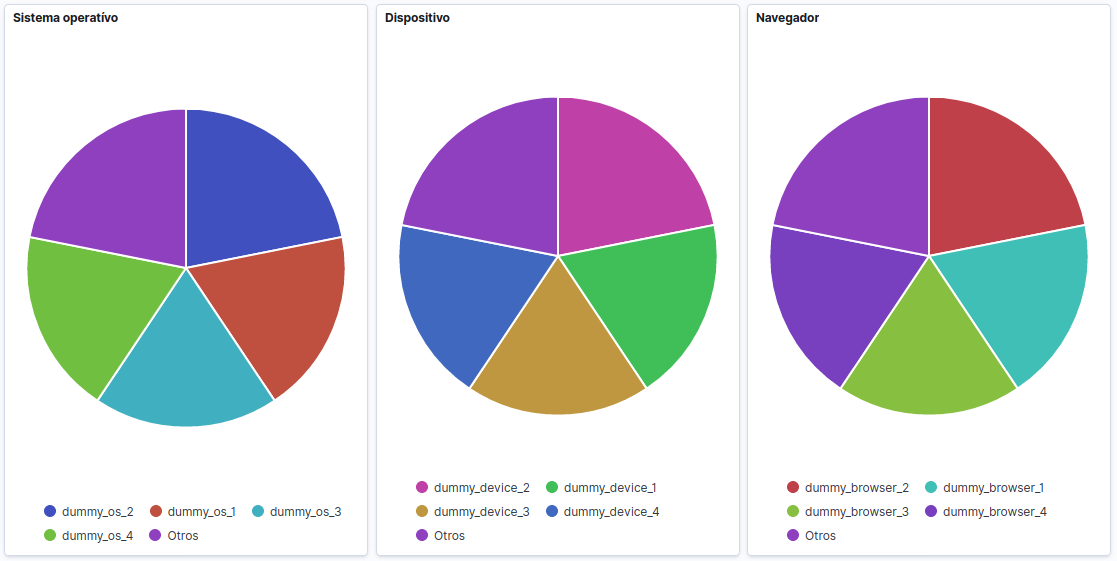
\includegraphics[width=11cm, keepaspectratio]{img/kibana_07_pie}
					\caption{Gráficas circulares para SO, Dispositivo y Navegador}
					\label{fig:kibana_pie}
				\end{figure}
				Tres gráficas circulares que representarán información acerca de los dispositivos que están siendo utilizados para acceder a la aplicación, filtra por sistema operativo, dispositivo y navegador.\\
				
				\begin{figure}[H]
					\centering
					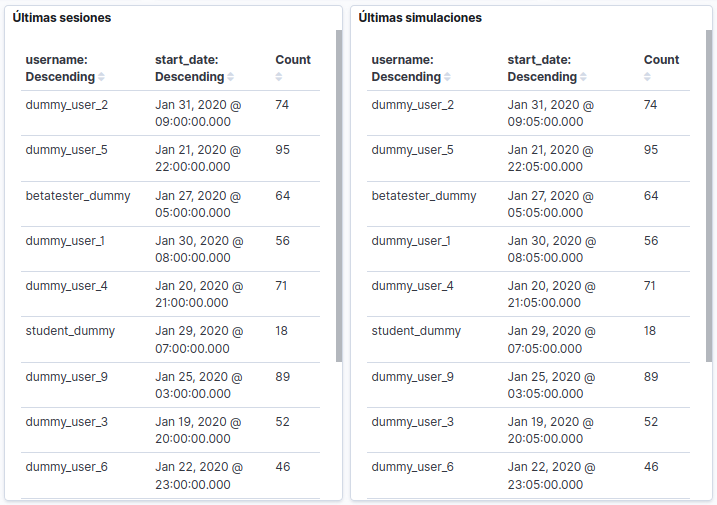
\includegraphics[width=10cm, keepaspectratio]{img/kibana_08_latest_event}
					\caption{Últimos eventos logueados}
					\label{fig:kibana_latestevent}
				\end{figure}
				Tabla de datos con los últimos registros de sesión y simulación para cada uno de los usuarios filtrados.\\
				
				Todas estas visualizaciones son interactivas y se puede filtrar por sus campos simplemente pulsando sobre ellas. Funcionalidad muy útil que no poseían las imagenes renderizadas que se generabane n el primer prototipo.\\
					
				Ya creadas las visualizaciones, solo quedará integrarlas en Kibotics al igual que se hizo con las generadas en Matplotlib. Para ello se creará una vista simple con la que se seleccionará a que tipo de analíticas se quiere acceder.

				\begin{figure}[H]
					\centering
					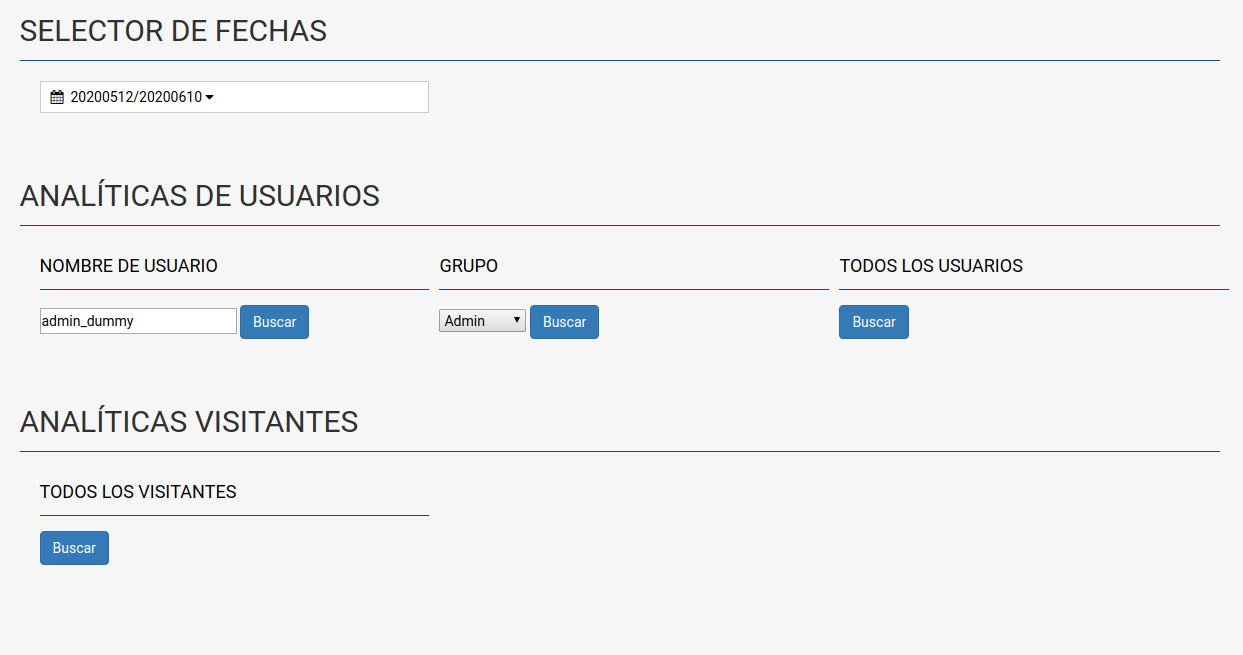
\includegraphics[width=12cm, keepaspectratio]{img/kibotics_analytics_menu.png}
					\caption{Menú de selección de analíticas en Kibotics}
					\label{fig:kibotics_analytics_menu}
				\end{figure}
			
				En esta vista se filtrará tanto por usuarios y grupos, como por fechas de las cuales queremos analíticas. Una vez filtrado, Django generará automaticamente una URL con los datos seleccionados en el Menú de Kibotics. Esta URL dinámica apuntará a las visualizaciones de nuestro servicio de Kibana y será devuelta por el contexto de Django hasta las plantillas que lo insertarán en un elemento HTML iFrame.
				
				
				\begin{figure}[H]
					\centering
					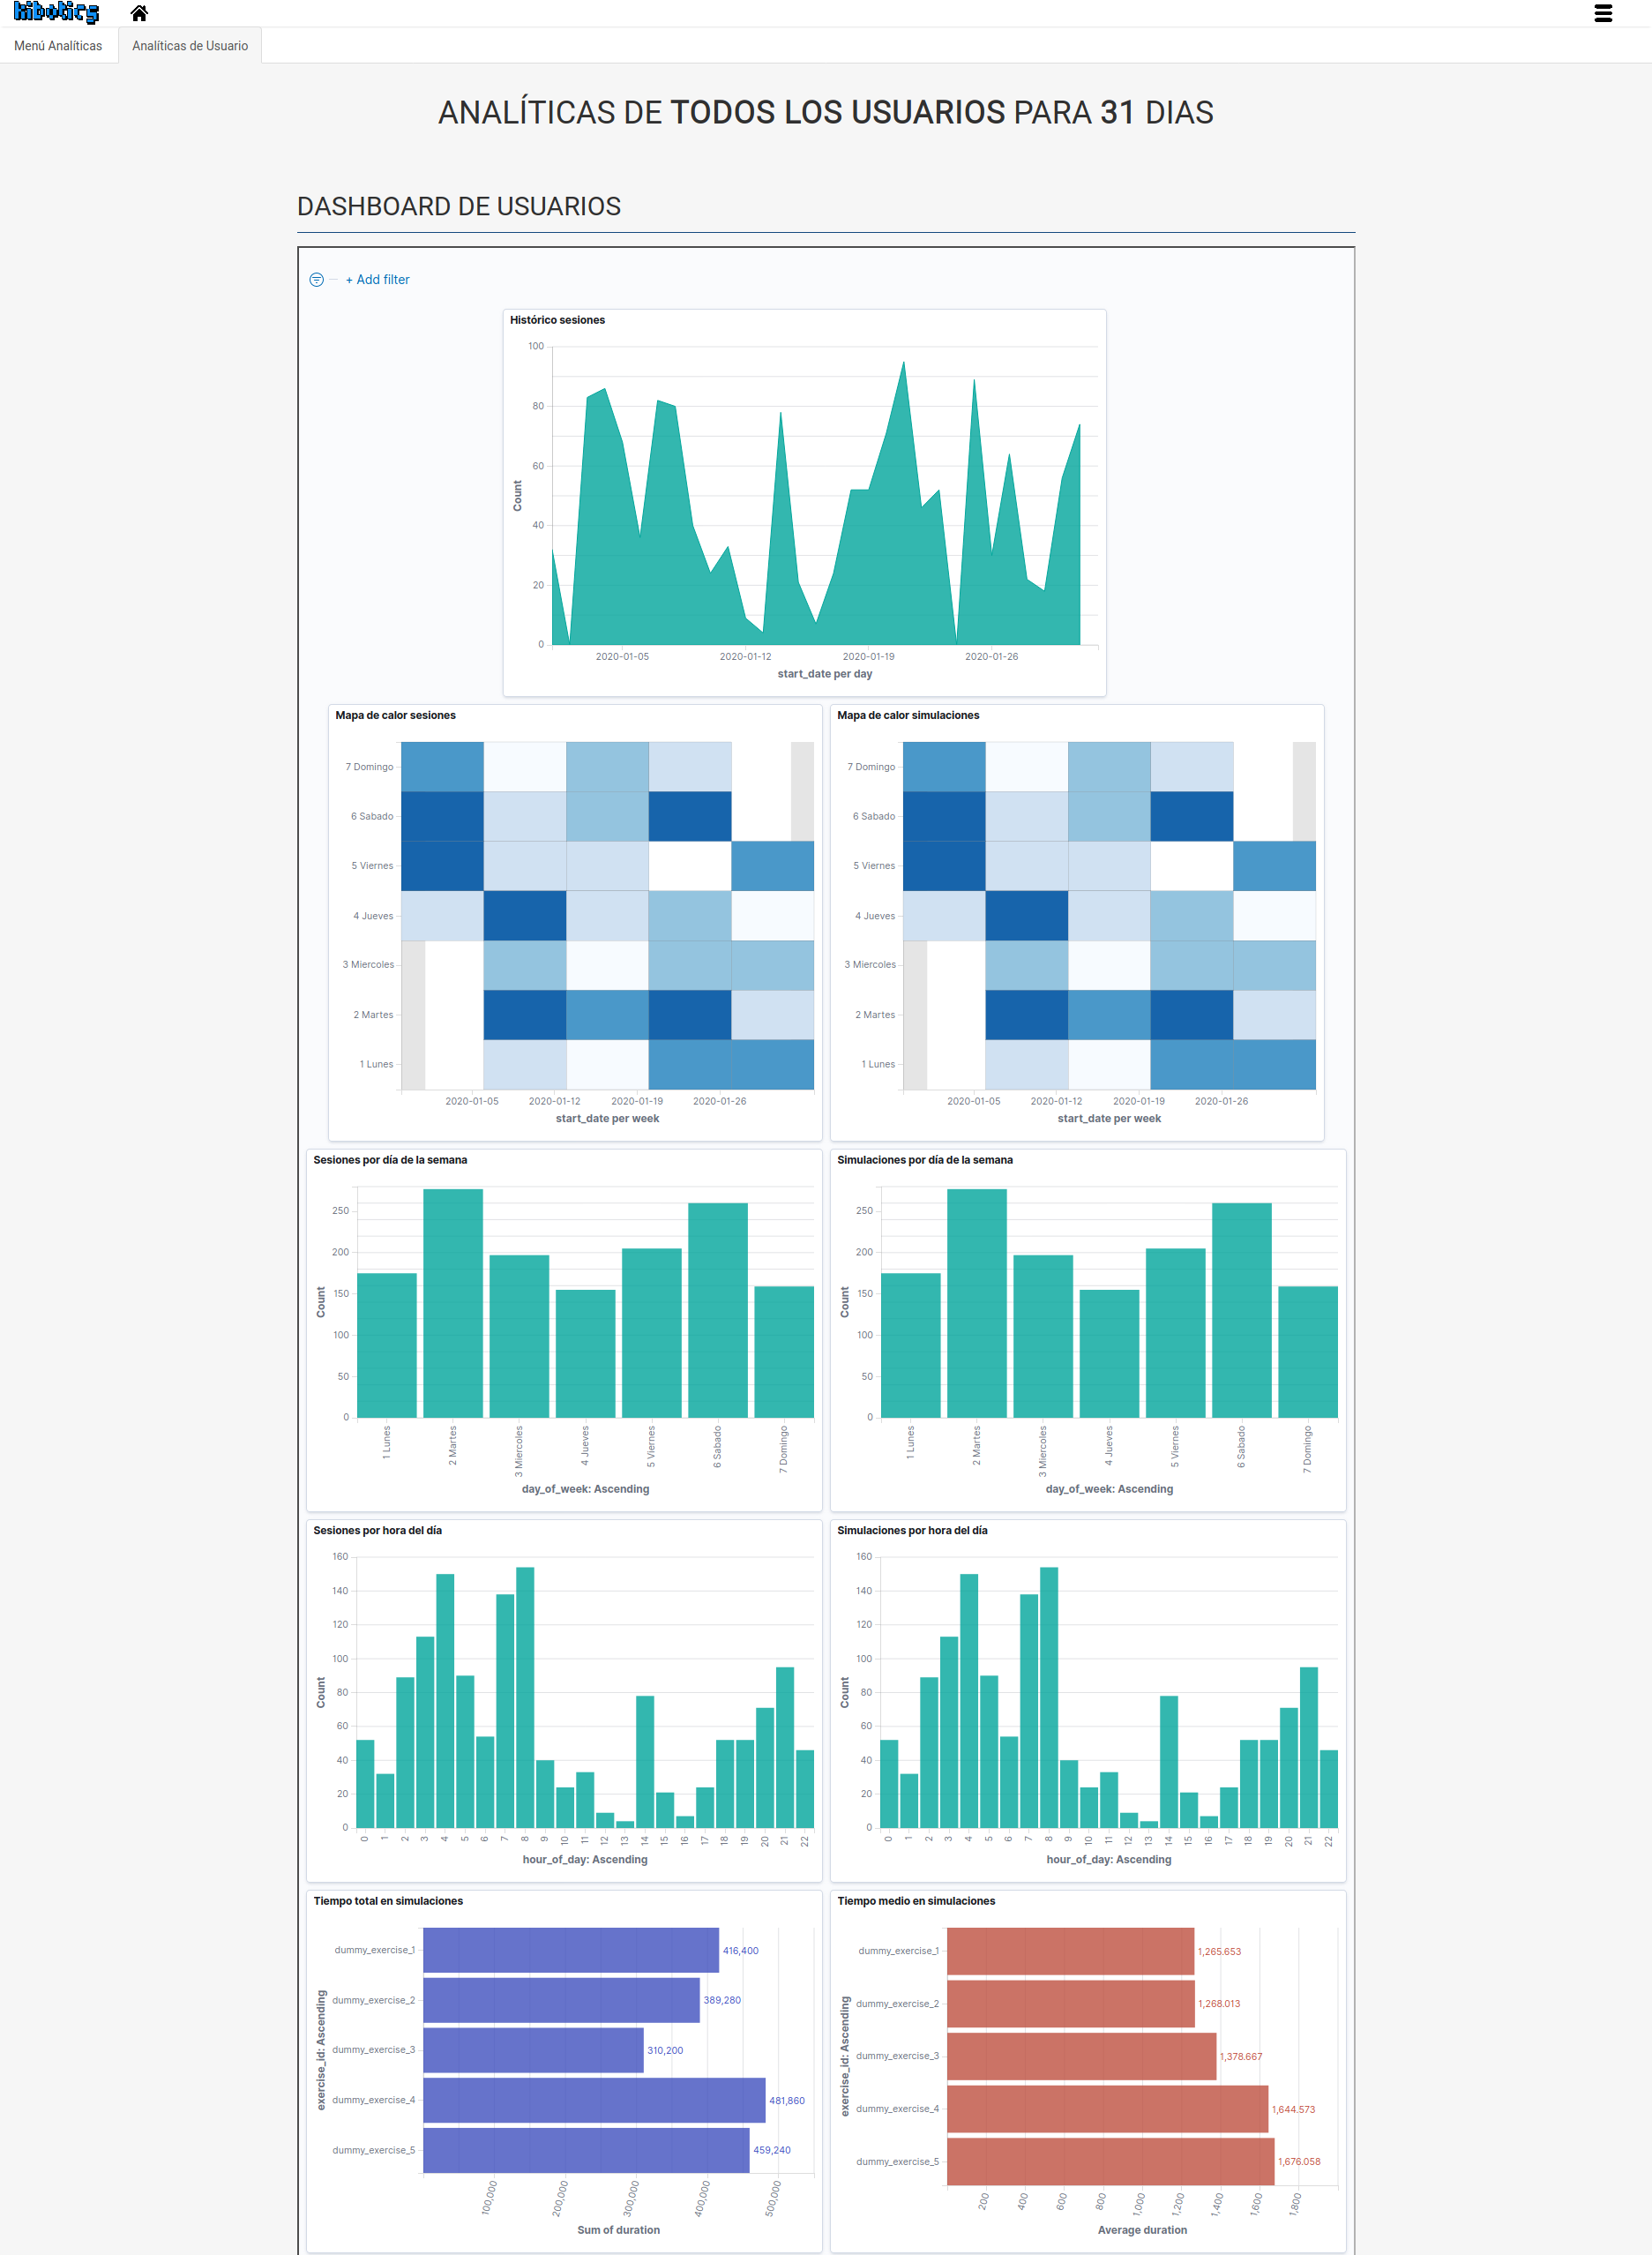
\includegraphics[width=10cm, keepaspectratio]{img/kibana_kibotics_01.png}
					\caption{Kibana en Kibotics parte 1}
					\label{fig:kibana_kibotics_01}
				\end{figure}
				\begin{figure}[H]
					\centering
					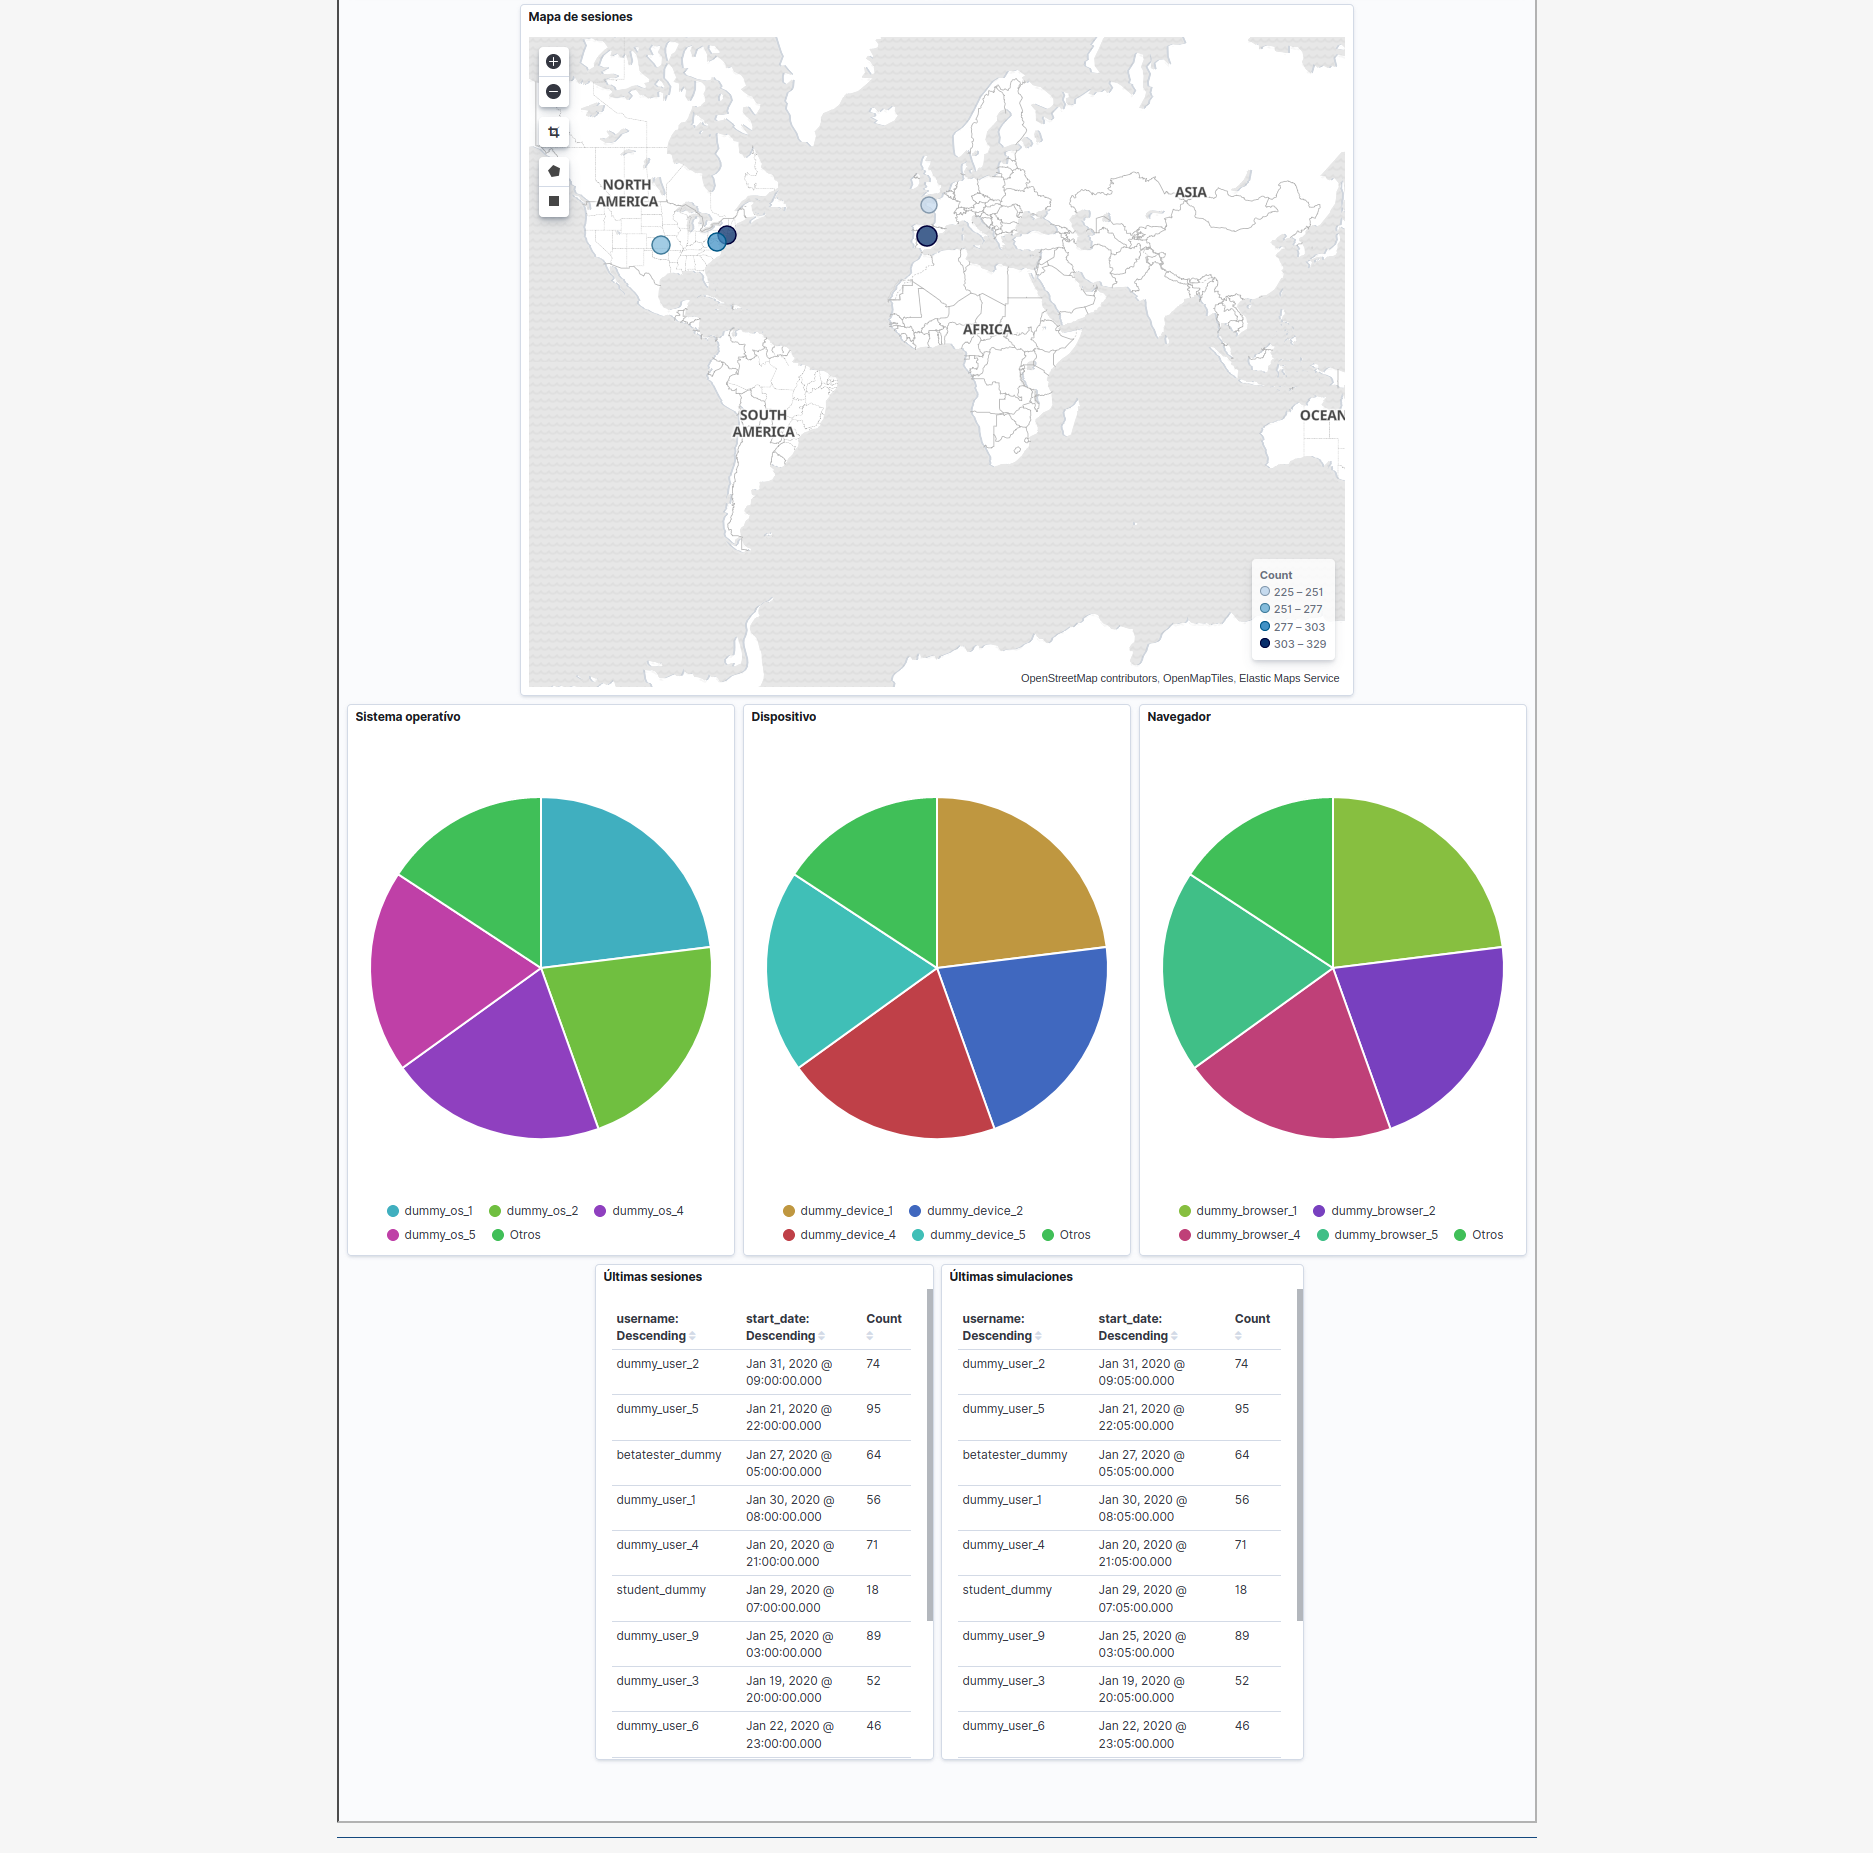
\includegraphics[width=10cm, keepaspectratio]{img/kibana_kibotics_02.png}
					\caption{Kibana en Kibotics parte 2}
					\label{fig:kibana_kibotics_02}
				\end{figure}
				\begin{figure}[H]
					\centering
					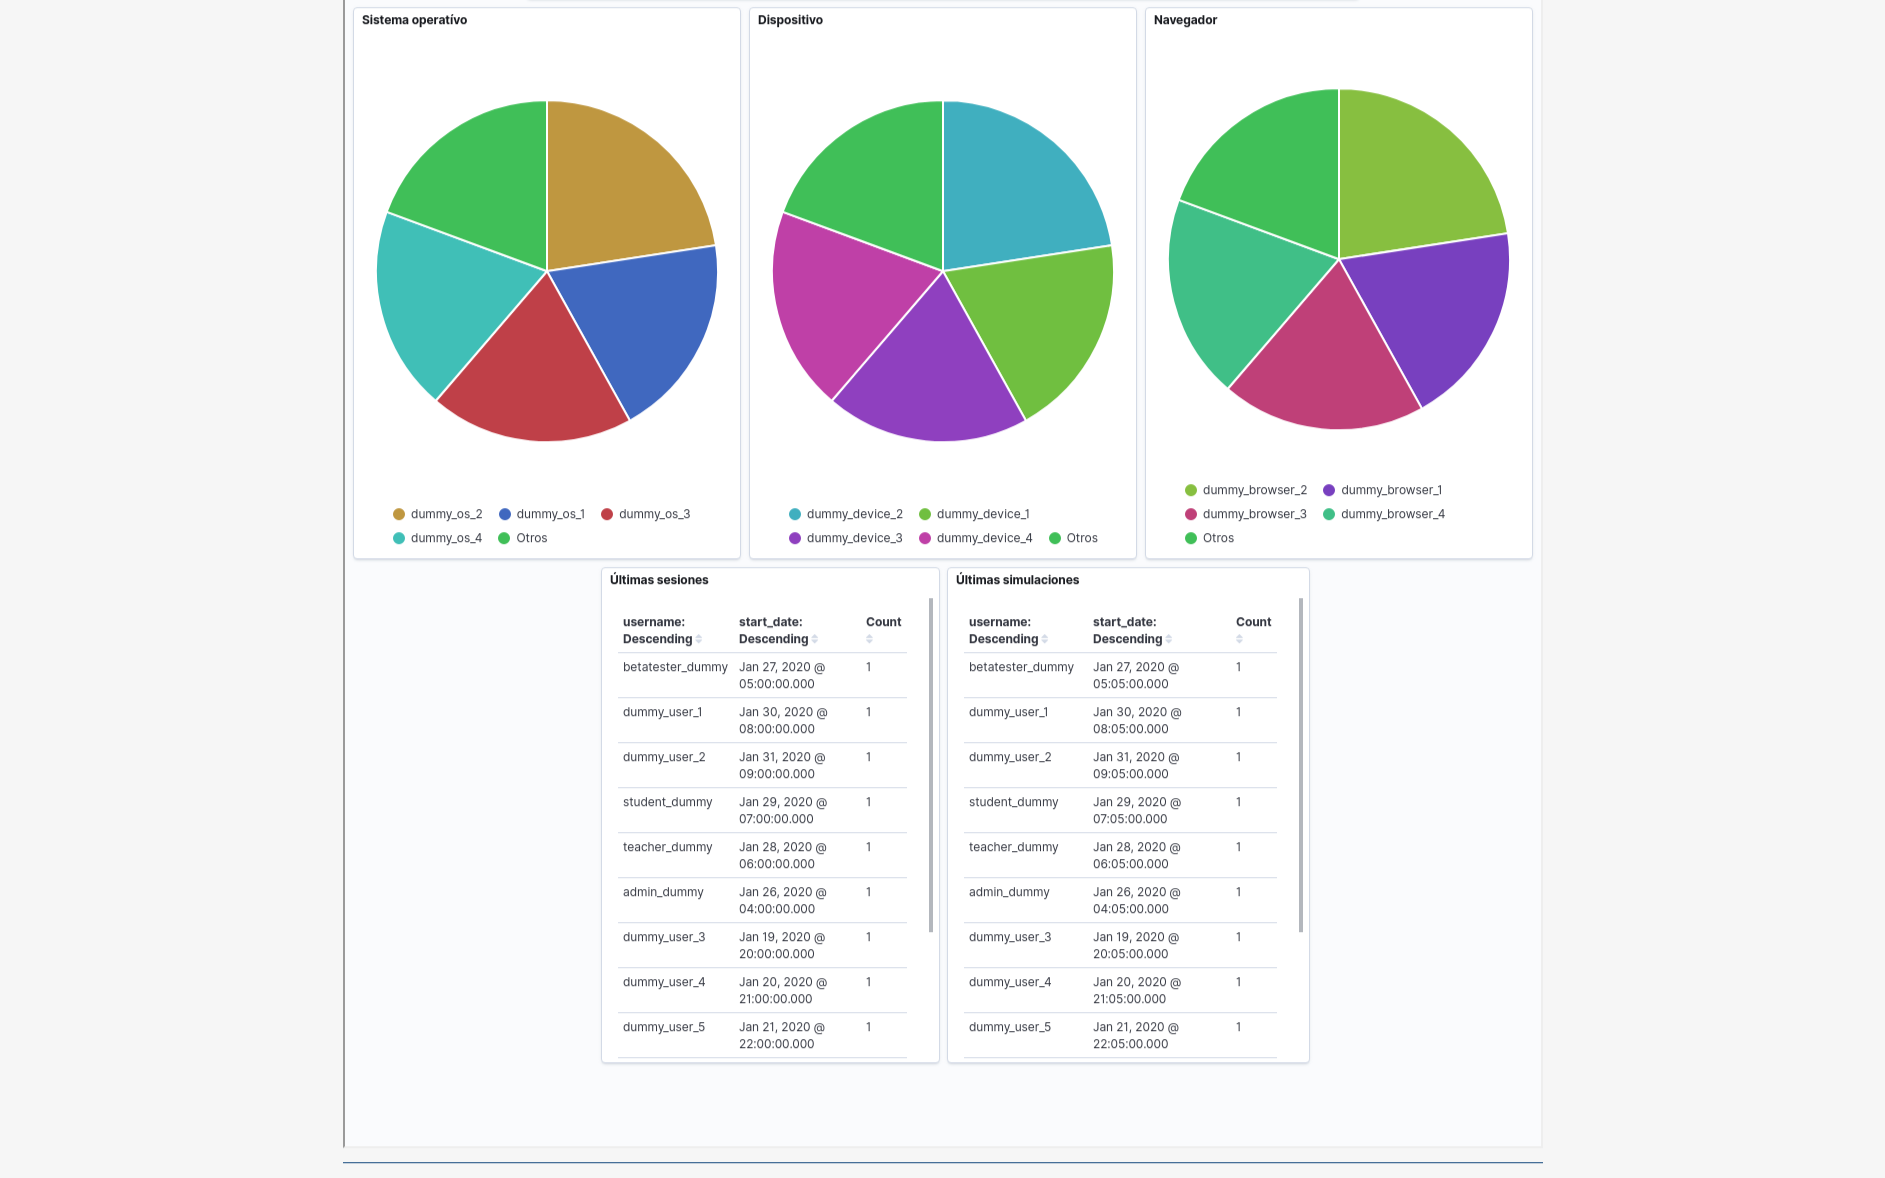
\includegraphics[width=10cm, keepaspectratio]{img/kibana_kibotics_03.png}
					\caption{Kibana en Kibotics parte 3}
					\label{fig:kibana_kibotics_03}
				\end{figure}
		\section{Despliegue en producción}
			(INCOMPLETO)
		\section{Generación de recusos de prueba para el desarrollo local}
			Para facilitar futuros desarrollos y ampliaciones de las mejoras de analíticas implementadas se han generado una serie de recursos para proveer al repositorio Github de herramientas.
			\subsection{Receta de instalación de ElasticSearch}
				Se ha incluido en el repositorio GitHub la receta necesaria para instalar la versión de ElasticSearch utilizada en producción.\\
				
				Con esto, se asegura que cualquier futuro desarrollador de la plataforma simplemente tenga que seguir la receta de instalación ahí explicitada para tener un entorno totalmente funcional.\\
				
				Actualmente la última versión estable de ElasticSearch es la versión 7.7.2, liberada el 3 de Junio de 2020. Por cuestión de fechas, en producción, actualmente se está utilizando la versión 7.6.2 del 31 de Marzo del 2020.
			\subsection{Creación de bases de datos Dummy para Elasticsearch}
				Para proporcionar a los futuros desarrolladores datos realistas con los que poder empezar a trabajar sin necesidad de crearlos de manera manual, se ha creado una base de datos dummy la cual ofrece una variedad de datos para todos los índices utilizados tanto en este proyecto, como en otros desarrollos paralelos.\\
				
				Para la creación de esta base de datos de pruebas, se generó mediante un script de Python el cual crea los índices y su estructura haciendo uso de la librería de que Elasticsearch proporciona para Python.\\
				
				El script creará todos los índices con sus respectivas estructuras y tipologías de datos, un ejemplo, para el índice de sesiones es:
				
				\begin{Verbatim}[tabsize=4]
# Import librería Elasticsearch
from elasticsearch import Elasticsearch
client = Elasticsearch()

...

# JSON con la estructura del índice
session_mapping = {
	"settings": {
		"number_of_shards": 1,
		"number_of_replicas": 0
	},
	"mappings": {
		"properties": {
			"username": {
				"type":"keyword"
			},
			"start_date":{
				"type":"date"
			},
			"end_date":{
				"type":"date"
			},
			"duration": {
				"type":"double"
			},
			"client_ip":{
				"type":"ip"
			},
			"browser": {
				"type":"keyword"
			},
			"device":{
				"type":"keyword"
			},
			"location": {
				"type": "geo_point"
			},
			"os":{
				"type":"keyword"
			}
		}
	}
}

# Creación del índice en ElasticSearch
client.indices.create(
	index="kibotics_session_log",
	body=session_mapping,
	ignore=400
)
				\end{Verbatim}
				
				Una vez creadas las estructuras de los índices, el siguiente paso es guardar todos los objetos con la información de prueba que se deseé guardar.\\
				
				Finalizada la ejecución del script ya tendríamos los datos en nuestro servicio local de Elasticsearch. Un problema que se encontró es que para ejecutar este script es necesaria la instalación de varias librerías. Para simplificar aún más la instalación de la base de datos se han generado una serie de documentos JSON con la estructura y datos que otros usuarios importarán a su servicio ElasticSearch.\\
				
				Estos documentos JSON se han generado haciendo uso de la herramienta elasticdump, la cual tiene una instalación muy sencilla:
							
				\begin{Verbatim}[tabsize=4]
$ sudo npm install elasticdump -g
				\end{Verbatim}
				
				Para la generación de los documentos de datos y mapeo se han ejecutado las siguientes sentencias para cada uno de los índices usados en Elasticsearch:

				\begin{Verbatim}[tabsize=4]
$ elasticdump --input=http://127.0.0.1:9200/"INDEX_NAME" 
			--output="./mapping_elasticseach.json" --type=mapping
			
$ elasticdump --input=http://127.0.0.1:9200/"INDEX_NAME" 
			--output="./data_elasticsearch.json" --type=data

				\end{Verbatim}
				
				Para la importación de estos ficheros en la base de datos, el desarrollador simplemente tendrá que instalar elasticdump y ejecutar un script bash el cual recorrerá y cargará todos los ficheros al servicio Elasticsearch local:
				
				\begin{Verbatim}[tabsize=4]
indexes="session simulation visit error classification ranking"
directory="./kibotics_dummy_es/"

for index in $indexes; do
	elasticdump --output=http://127.0.0.1:9200/"kibotics_"$index"_log" 
		--input=$directory"mapping_"$index"_es.json" --type=mapping

	elasticdump --output=http://127.0.0.1:9200/"kibotics_"$index"_log" 
		--input=$directory"data_"$index"_es.json" --type=data
done
				\end{Verbatim}
			\subsection{Receta de instalación de Kibana}
			Para completar la instalación de recursos del Stack ELK utilizados en el proyecto se ha añadido la receta de instalación de Kibana.\\
			
			Actualmente la última versión estable de Kibana es la versión 7.7.1, liberada el 3 de Junio de 2020. Por cuestión de fechas, en producción, actualmente se está utilizando la versión 7.7.0 del 13 de Mayo del 2020.
			
			\subsection{Creación de bases de datos Dummy para Kibana}
			El proceso de exportación e importación de datos de prueba para kibana es sencillo pues la propia interfaz gráfica de Kibana nos proporciona una herramienta para realizarlo.
			
			\begin{figure}[H]
				\centering
				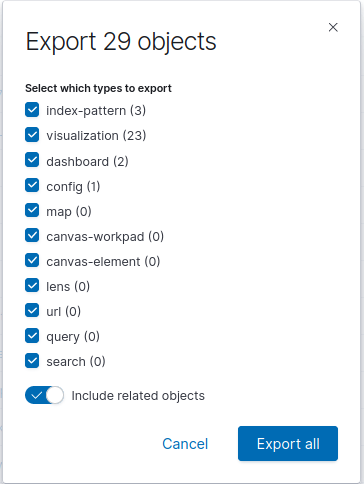
\includegraphics[width=7.5cm, keepaspectratio]{img/export_kibana.png}
				\caption{Exportación en interfaz Kibana.}
				\label{fig:export_kibana}
			\end{figure}
		
			Esta herramienta nos generará un fichero NDJSON similar a la estructura JSON con los patrones de índices creados, así como las visualizaciones, tablas o campos scripted guardados en Kibana.\\
			
			Para que un futuro desarrollador importe estos datos simplemente podrá hacerlo por la interfaz gráfica de Kibana. Para unificar la metodología y ya que en el servidor de pre-producción/producción no se dispone de esta interfaz gráfica, esta también se puede realizar mediante la siguiente sentencia:\\
			

			
			\begin{Verbatim}[tabsize=4]
$ curl -X POST "localhost:5601/api/saved_objects/_import" -H "kbn-xsrf: true" 
	--form file=@kibotics_dummy_kibana.ndjson
			\end{Verbatim}
			
			


	\chapter{CONCLUSIONES}
		Finalmente, en este último capítulo se exponen las conclusiones alcanzadas, así como las competencias adquiridas durante la realización de este proyecto. Además, se plantean futuros trabajos de ampliación y mejora sobre el software desarrollado.
		\section{Conclusiones finales}
			Repasando lo definido en el capítulo 2, el principal objetivo de este proyecto es crear una herramienta en la que visualizar y analizar el estado de la aplicación Web Kibotics Webserver. Este objetivo se ha cumplido, se ha diseñado, desarrollado y testeado un módulo de analíticas en el que visualizar estos datos de uso de la aplicación.\\
			
			Adicionalmente a esto, se ha mejorado el sistema de registro de logs de la aplicación. Eliminando los ficheros de log indexados por días y creando una base de datos en ElastiSearch dividida en distintos índices sobre los que se registran variedad de eventos. Aumentando así la escalabilidad de este proceso de registro de logs y eventos, con lo que se consigue que esta sea una solución robusta y duradera.
		\section{Competencias adquiridas}
			En esta sección se enumeran las principales habilidades que se han adquirido en el desarrollo de este proyecto:
			\begin{itemize}
				\item Django y Python como herramientas muy potentes y accesibles para el desarrollo Web. Además, gracias a las librerías de las que estas disponen, son herramientas muy versátiles.\\
				
				\item Despliegue e implementación de diferentes tipos de bases de datos en un proyecto real. Importancia de la información para monitorizar un servicio Web.\\
				
				\item El Stack ELK, ha sido una herramienta muy potente de la que he aprendido como es integrar varias tecnologías para crear un producto complejo, interconectado e interesante.\\
				
				\item GitHub, durante el desarrollo de este proyecto este repositorio ha estado siempre presente junto a la filosofía 'release often, release soon'.\\
				
				\item Trabajar en un software actualmente productivo sobre el que desarrollar para crear nuevas funcionalidades. Saber que no se dispone de los pasos a seguir y tener que investigar diferentes tecnologías para encontrar una solución óptima.\\
				 
				\item Una primera toma en contacto con el análisis de datos, sobre el que tendré que seguir aprendiendo y descubriendo nuevas tecnologías.\\
			\end{itemize}
			
		\section{Competencias empleadas}
			En el transcurso de este proyecto se han utilizado muchos de los conocimientos y habilidades adquiridos en el Grado, en especial en las asignaturas relacionadas con el desarrollo web. A continuación se enumerarán estas y otras asignaturas que me han aportado los conocimientos necesarios:
			
			\begin{itemize}
				\item Informática I, con el lenguaje ’Picky’ donde aprendí los fundamentos básicos de programación.	
				
				\item Informática II, en la que se llevaron a cabo proyectos más complejos, centrado en el aprendizaje de punteros y estructuras de datos complejas como tablas Hash. Haciendo uso del lenguaje ADA.	
						
				\item Protocolos de Transmisión de Audio y Vídeo en Internet, primera toma de contacto con Python y GithHub, herramientas imprescindibles para el desarrollo de este proyecto.
							
				\item Gráficos y visualización 3D, introducción al desarrollo web, centrado en JavaScript y el canvas HTML.			
			
				\item Construcción de Servicios y Aplicaciones Audiovisuales en Internet, asignatura muy importante en la que se profundizó en las 3 tecnologías web principales: JavaScript, HTML y CSS.
				
				\item Laboratorios en Tecnologías y Aplicaciones Web, ampliación de la anterior asignatura en la que aprendí a trabajar con frameworks web como NodeJS o Django, base de Kibotics Webserver.
			\end{itemize}
			
			
		\section{Trabajos futuros}
			En esta sección se proponen una serie de mejoras o ampliaciones con las que aumentar la funcionalidad del módulo de analíticas desarrollado:
			
			\begin{itemize}
				\item Kibotics Webserver es una aplicación grande y en constante ampliación, añadir mas sondas con las que tener la aplicación controlada será recomendable. Con estas nuevas sondas será necesaria la creación de nuevos índices y visualizaciones.\\
				
				\item Actualmente los datos almacenados en ElasticSearch solo pueden ser analizados accediendo al módulo desarrollado. Una herramienta automática que analice estos datos sería muy interesante para controlar, por ejemplo que todos los ejercicios están siendo accedidos y los tiempos de desarrollo de los usuarios no son demasiado elevados.\\
				
				\item El Stack ELK posee, además de ElasticSeach y Kibana, otras herramientas muy interesantes como Logstash y Beats. Las cuales pueden dotar a ElasticSeach de nuevos datos procedentes de otras fuentes, como por ejemplo, logs del servidor con los que controlar los accesos que sufre la herramienta.\\
				
				\item Explorar otras mejoras de integración a la Web De kibotics, ya que el Iframe no es algo ideal que tener en un servicio productivo por motivos de seguridad.\\
							
				\item El Stack ELK es un software en constante evolución la cual añade nuevas y mejores funcionalidades constantemente. Mantener las versiones del software actualizadas es recomendable.\\
				
				\item Al proporcionar información muy sensible sobre el servicio, aumentar la seguridad en el servidor para acceder a estos datos es necesario.\\
			\end{itemize}
		
	\chapter{REFERENCIAS}
	Django
https://www.djangoproject.com/
	Django MVC
https://uniwebsidad.com/libros/django-1-0/capitulo-5/el-patron-de-diseno-mtv

	HTML 
	https://uniwebsidad.com/libros/xhtml/capitulo-1/breve-historia-de-html
	https://www.w3schools.in/html-tutorial/history/
	
	SQLite
	https://www.sqlite.org/about.html
	
	Elasticsearch
	http://www.arquitectoit.com/elasticsearch/que-es-elasticsearch/
	https://www.ionos.es/digitalguide/servidores/configuracion/que-es-elasticsearch/
	https://www.elastic.co/guide/en/elastic-stack-get-started/7.6/get-started-elastic-stack.html\#install-elasticsearch
	
	Matplotlib
	https://matplotlib.org/
	
	kibana
	https://www.elastic.co/es/what-is/kibana

	Elasticdump\\
	https://www.npmjs.com/package/elasticdump
	\chapter{IMPLEMENTACIÓN DE MEJORAS PARA HERRAMIENTAS DE GESTIÓN}
		\section{Asignación de permisos individuales}
\end{document}